%  ----------------------------------------------------------------------------
%
%       Copyright (for the thesis) 2009 by [author - insert yourself]
%
%       This thesis is published under the
%       Creative Commons Attribution-No Derivative Works 3.0 Austria License
%       as detailed at http://creativecommons.org/licenses/by-nd/3.0/at/
%
%  ----------------------------------------------------------------------------
%  Template credits and license:
%  ----------------------------------------------------------------------------
%
%       "Fakultät für Informatik" diploma/master thesis template 2008
%
%       based upon "Diploma thesis template 2005" by lukas.silberbauer(at)gmx.at
%       based upon "Diplomarbeit mit LaTeX" by Tobias Erbsland
%       incorporating a title page by Informatik-Forum user "Baby"
%       polished and ported to the TU fonts package by Jakob Petsovits
%
%       published under the terms of
%
%  ----------------------------------------------------------------------------
%  "THE BEER-WARE LICENSE":
%  <lukas.silberbauer(at)gmx.at> wrote this file. As long as you retain this
%  notice you can do whatever you want with this stuff. If we meet some day,
%  and you think this stuff is worth it, you can buy me (us) a beer in return.
%  ----------------------------------------------------------------------------
%
%  (end of template credits)
%

%
% Variablen, die fürs Deckblatt verwendet werden.
% Die grobe Dokumentenstruktur findet sich übrigens ganz unten in dieser Datei.
%
\newcommand{\thesistype}{DIPLOMARBEIT}
\newcommand{\thesistitle}{Effektivit\"{a}tsanalyse des c-Collision Protokolls}
\newcommand{\thesissubtitle}{ als gewichteter Datenbalancierer in einem parallelen Out-of-Core Renderer}

\newcommand{\thesisauthor}{Timo Wiesemann}
\newcommand{\matrikelnr}{6015295}
\newcommand{\zuerlangendertitel}{Diplom-Informatiker}
\newcommand{\studium}{Informatik}

\newcommand{\institut}{Heinz Nixdorf Institut Paderborn}
\newcommand{\institutsuni}{Universit\"{a}t Paderborn} % disabled by default
\newcommand{\betreuer}{Dr. Matthias Fischer}
\newcommand{\assistent}{Dipl.-Inf. Tim Suess}

%
% Globale Weichenstellungen fürs ganze Dokument.
%
\documentclass[%
  pdftex,%              PDFTex verwenden
  a4paper,%             A4 Papier
  oneside,%             Einseitig
  bibtotocnumbered,%    Literaturverzeichnis nummeriert einfügen
  idxtotoc,%            Index ins Verzeichnis einfügen
  %liststotoc,
  liststotocnumbered,
  halfparskip,%         Europäischer Satz mit abstand zwischen Absätzen
  chapterprefix,%       Kapitel anschreiben als Kapitel
  %headsepline,%         Linie nach Kopfzeile
  %footsepline,%         Linie vor Fusszeile
  12pt%                 Größere Schrift, besser lesbar am Bildschrim
]{scrbook}


%
% Paket für die Indexerstellung.
%
\usepackage{makeidx}

%
% Paket für Übersetzungen ins Deutsche
%
%\usepackage[english, german]{babel}
\usepackage[german, english, ngerman]{babel}


%
% Paket, um \today auch im Format dd.mm.yyyy anzeigen zu können
%  (für die Titelseite, mit \numdate)
%
\usepackage[german]{isodate}

%
% Pakete um Latin1 Zeichnensätze verwenden zu können und die dazu
%  passenden Schriften.
%
%\usepackage{ucs}
\usepackage[utf8]{inputenc}
\usepackage[T1]{fontenc}

%
% Paket zum Erweitern der Tabelleneigenschaften
%
\usepackage{array}

\usepackage{appendix}

%
% Paket um Grafiken einbetten zu können
%
\usepackage{graphicx}


%
% Zeilenabstand einstellen
%
\usepackage{setspace}
\onehalfspacing
%\doublespacing


%\setlength{\baselineskip}{24pt}
%\renewcommand{\baselinestretch}{1.5}


%
% define variables
%
\def\maintitle#1{\gdef\maintitle{#1}}
\def\subtitle#1{\gdef\subtitle{#1}}

%
% Zeilenumbruch bei Bildbeschreibungen.
%
\setcapindent{1em}

%
% Kopf- und Fußzeilen
%
\pagestyle{headings}

%
% mathematische symbole aus dem AMS Paket.
%
\usepackage{amsmath}
\usepackage{amssymb}

%
% Type 1 Fonts für bessere darstellung in PDF verwenden.
%
\usepackage{mathptmx}           % Times + passende Mathefonts
%\usepackage[scaled=.92]{helvet} % skalierte Helvetica als \sfdefault
\usepackage{courier}            % Courier als \ttdefault
\usepackage{tufonts}            % TU-Schriften als \sfdefault

%
% Spezielle Schrift verwenden.
%
\renewcommand{\encodingdefault}{T1}
\renewcommand{\familydefault}{\rmdefault}
\renewcommand{\bfdefault}{db}   % bold would be too bold, use demibold instead
\renewcommand{\mddefault}{l}    % use TU Light, looks better than medium weight



%
% Paket um Textteile drehen zu können
%
\usepackage{rotating}


%
% Für Acronyme
%
\usepackage{acronym}

%
% Package für Farben im PDF
%
\usepackage{color}

%
% Paket für Links innerhalb des PDF Dokuments
%
%\definecolor{LinkColor}{rgb}{0,0,0.5}
\definecolor{LinkColor}{rgb}{0,0,0}

\usepackage[
pdfauthor={\thesisauthor},
bookmarks=true, % PDF bookmarks allowed. NB! The level depth of bookmarks is the same as in the TOC.
unicode=true, % PDF bookmarks in Unicode.
bookmarksnumbered=true, % Section numbers in PDF bookmarks.
bookmarksopenlevel=1, % The open level in PDF bookmarks.
hyperindex=true, % Hyperlinked index.
plainpages=false, % Name arabic and roman page numbers differently.
colorlinks=true, % Links are marked as coloured text, not coloured box.
linkcolor=linkc, % The colour for in-document links (e.g. in the table of contents).
linkcolor=linkc, % The colour for in-document links (e.g. in the table of contents).
citecolor = citec, % The colour for bibliographic citations.
urlcolor=urlc, % The colour for hyperlinks to the Net.
pdfpagelayout=OneColumn % Continuous page scrolling.
]{hyperref}
\hypersetup{
  colorlinks=true,
  linkcolor=LinkColor,
  citecolor=LinkColor,
  filecolor=LinkColor,
  menucolor=LinkColor,
  pagecolor=LinkColor,
  urlcolor=LinkColor
}

%
% Paket um Listings sauber zu formatieren.
%
\usepackage[savemem]{listings}
\lstloadlanguages{TeX}

%
% macros für externalisierung der tikz-bilder
%
\newif\iffinal % introduce a switch for draft vs. final document
%\finaltrue % use this to compile the final document

% [more preamble that in my case also uses \iffinal for other stuff]

\usepackage{tikz}
\pgfrealjobname{thesis} % <-- NOTE: this needs to be the real document's basename
                        %     (else you'll only get an empty output file)

\iffinal
  \newcommand{\inputTikZ}[1]{%
    \input{#1.tikz}%
  }
\else
  \newcommand{\inputTikZ}[1]{%
    \beginpgfgraphicnamed{#1-external}%
    \input{#1.tikz}%
    \endpgfgraphicnamed%
  }
\fi
%
% ---------------------------------------------------------------------------
% Listing Definitionen für PHP Code
%
\definecolor{lbcolor}{rgb}{0.85,0.85,0.85}
\lstset{language=[LaTeX]TeX,
  numbers=left,
  stepnumber=1,
  numbersep=5pt,
  numberstyle=\tiny,
  breaklines=true,
  breakautoindent=true,
  postbreak=\space,
  tabsize=2,
  basicstyle=\ttfamily\footnotesize,
  showspaces=false,
  showstringspaces=false,
  extendedchars=true,
  backgroundcolor=\color{lbcolor}
}
% ---------------------------------------------------------------------------
% Selbentrennung
% ---------------------------------------------------------------------------
\hyphenation{Bild-ra-ten Mo-dell Mo-dells Mo-del-le Spei-cher-ver-wal-tung ge-o-me-tri-e pa-ral-lel pa-ral-le-len Ope-ra-ti-on Ope-ra-ti-o-nen Ap-pro-xi-ma-ti-on ent-sprech-en-den Netz-werk er-reicht}
\sloppy

%----------------------------------------------------------------------------
% Tabellenlinien und sonstige nützliche Dinge
% ---------------------------------------------------------------------------
\usepackage{booktabs}

% ---------------------------------------------------------------------------
% Neue Umgebungen
% ---------------------------------------------------------------------------

\newenvironment{ListChanges}%
  {\begin{list}{$\diamondsuit$}{}}%
  {\end{list}}

%
% Index erzeugen
%
\makeindex

\usepackage{tikz}
\usetikzlibrary{arrows,shadows} % for pgf-umlsd

\usepackage{soul} % hereby we are able to \hl == highlight some strings, or to \ul underline specials

%\usepackage[underline=true,rounded corners=false]{pgf-umlsd} % changed to following parameter-values:
\usepackage[underline=false,rounded corners=true]{pgf-umlsd}

% todo notes, add disbale to remove them. BUT: need to remove the toc-insertion manually
%\usepackage[colorlinks]{hyperref}
\usepackage[colorinlistoftodos, shadow]{todonotes}

\usepackage{pgfplots}

\usepackage{algorithm}
\usepackage{algorithmic, algorithmic-fix}
\renewcommand{\algorithmiccomment}[1]{//\textit{#1}}

\usepackage{caption}
\newenvironment{Bild}
  {\par\noindent\minipage{\textwidth}\centering}
  {\endminipage}

\usepackage{verbatim} 

%%%%%%%%%%%%%%%%%%%%%%%%%%%%%%%%%%%%%%%%%%%%%%%%%%%%%%%%%%%%%%%%%%%%%%
%
% Document structure
%
%%%%%%%%%%%%%%%%%%%%%%%%%%%%%%%%%%%%%%%%%%%%%%%%%%%%%%%%%%%%%%%%%%%%%%

\begin{document}
\renewcommand\contentsname{Inhaltsverzeichnis}
\renewcommand\listfigurename{Abbildungsverzeichnis}
\renewcommand\listtablename{Tabellenverzeichnis}
\renewcommand{\listalgorithmname}{Algorithmenverzeichnis}

\pagenumbering{alph}
%  ----------------------------------------------------------------------------
%
%       Copyright (for the thesis) 2009 by [author - insert yourself]
%
%       This thesis is published under the
%       Creative Commons Attribution-No Derivative Works 3.0 Austria License
%       as detailed at http://creativecommons.org/licenses/by-nd/3.0/at/
%
%  ----------------------------------------------------------------------------
%  Template credits and license:
%  ----------------------------------------------------------------------------
%
%       "Fakultät für Informatik" diploma/master thesis template 2008
%
%       based upon "Diploma thesis template 2005" by lukas.silberbauer(at)gmx.at
%       based upon "Diplomarbeit mit LaTeX" by Tobias Erbsland
%       incorporating a title page by Informatik-Forum user "Baby"
%       polished and ported to the TU fonts package by Jakob Petsovits
%
%       published under the terms of
%
%  ----------------------------------------------------------------------------
%  "THE BEER-WARE LICENSE":
%  <lukas.silberbauer(at)gmx.at> wrote this file. As long as you retain this
%  notice you can do whatever you want with this stuff. If we meet some day,
%  and you think this stuff is worth it, you can buy me (us) a beer in return.
%  ----------------------------------------------------------------------------
%
%  (end of template credits)
%

\selectlanguage{german}
\begin{titlepage}
\fontfamily{fts}\selectfont

\vspace*{-0.75cm}

\begin{minipage}[t]{0.3\linewidth}
\begin{flushleft}
\begin{center}
 \includegraphics[scale=0.75]{images/Logo_Uni_Paderborn.pdf}
 % Logo_Uni_Paderborn.pdf: 442x117 pixel, 72dpi, 15.59x4.13 cm, bb=0 0 442 117
\end{center}

\end{flushleft}
\end{minipage}

\vspace{1.0cm}

\begin{center}
\dmseries\huge{\thesistitle \\ \thesissubtitle}
\end{center}

\vspace{0.5cm}

\renewcommand{\bigskip}{\vspace*{0.43cm}}

\begin{center}
\begin{Large}\thesistype \end{Large} \bigskip \\
\begin{normalsize}zur Erlangung des akademischen Grades \end{normalsize} \bigskip \\
\begin{Large}\dmseries\zuerlangendertitel\end{Large} \bigskip \\
\begin{normalsize}im Rahmen des Studiums\end{normalsize} \bigskip \\
\begin{large}\dmseries\studium\end{large} \bigskip \\
\begin{normalsize}ausgef\"{u}hrt von \end{normalsize} \bigskip \\
\begin{large}\dmseries\thesisauthor\end{large} \\
\begin{normalsize}Matrikelnummer: \matrikelnr\end{normalsize} \\
\end{center}

\begin{flushleft}
am: \\ \textit{\institut} \\
%\small{der \institutsuni} \\
\end{flushleft}


\begin{flushleft}
\smallskip
Betreuung: \\
\textit{Betreuer: \betreuer} \\
\textit{Mitwirkung: \assistent}
\end{flushleft}

\date{\today}
\numdate

\footnotesize
\vspace{1.5cm}

\begin{flushleft}
\begin{tabbing}%
%Wien, \today & \hspace*{0.5cm} & \underline{\hspace*{5.2cm}} & \hspace*{1.0cm} & \underline{\hspace*{5.2cm}}\\
%                       &                 &         Unterschrift Verfasserin  & & Unterschrift Betreuer
\hspace{4.5cm} \= \hspace{5cm} \= \hspace{5cm} \kill
\textit{Paderborn, \today} \> \underline{\hspace*{5cm}} \> \hspace{0.8cm} \underline{\hspace*{5cm}} \\
     \> \hspace{0.1cm} (Unterschrift Verfasser/in) \> \hspace{1.0cm} (Unterschrift Betreuer/in) \\
\end{tabbing}
\end{flushleft}

\vspace{0.9cm}

\begin{minipage}[b]{1.0\linewidth}
\begin{center}
\underline{\hspace*{15.5cm}}
\scriptsize{
Technische Universit\"{a}t Wien \\
A-1040 Wien \hspace{0.5cm} Karlsplatz 13 \hspace{0.5cm} Tel. +43/(0)1/58801-0 \hspace{0.5cm} http://www.tuwien.ac.at
}
\end{center}
\end{minipage}

\vspace*{-2.5cm}

\end{titlepage}

%
% EOF
%

\newpage
\thispagestyle{empty}
Wiesemann, Timo \\

\begin{center}
  \textit{\textbf{Erklärung}}
\end{center}

\hspace*{60mm}\\

Hiermit versichere ich, die Diplomarbeit selbstständig verfasst und dabei keine anderen als die angegebenen und bei Zitaten kenntlich gemachten Quellen als Hilfsmittel verwendet zu haben.
\bigskip

Außerdem verpflichte ich mich, ein drittes Exemplar meiner Diplomarbeit 5 Jahre aufzubewahren und sie auf Verlangen jederzeit herauszugeben.\\
\\
Die Frist beginnt am \hrulefill\ (Tag der Abgabe der Arbeit).\\
\\
\\
\\
\\
\begin{minipage}{25cm}
  \begin{flushright}
    \begin{center}
      \rule{7cm}{0.2mm}\\
      Datum, Unterschrift
      \end{center}
  \end{flushright}
\end{minipage}
\newpage


\selectlanguage{german}
\pagenumbering{roman}
\setcounter{page}{1}

\listoftodos
\addcontentsline{toc}{chapter}{ToDoList}


\tableofcontents
\addcontentsline{toc}{chapter}{Inhaltsverzeichnis}

\pagenumbering{arabic}
\setcounter{page}{1}

%  ----------------------------------------------------------------------------
%
%       Copyright (for the thesis) 2009 by [author - insert yourself]
%
%       This thesis is published under the
%       Creative Commons Attribution-No Derivative Works 3.0 Austria License
%       as detailed at http://creativecommons.org/licenses/by-nd/3.0/at/
%
%  ----------------------------------------------------------------------------
%  Template credits and license:
%  ----------------------------------------------------------------------------
%
%       "Fakultät für Informatik" diploma/master thesis template 2008
%
%       based upon "Diploma thesis template 2005" by lukas.silberbauer(at)gmx.at
%       based upon "Diplomarbeit mit LaTeX" by Tobias Erbsland
%       incorporating a title page by Informatik-Forum user "Baby"
%       polished and ported to the TU fonts package by Jakob Petsovits
%
%       published under the terms of
%
%  ----------------------------------------------------------------------------
%  "THE BEER-WARE LICENSE":
%  <lukas.silberbauer(at)gmx.at> wrote this file. As long as you retain this
%  notice you can do whatever you want with this stuff. If we meet some day,
%  and you think this stuff is worth it, you can buy me (us) a beer in return.
%  ----------------------------------------------------------------------------
%
%  (end of template credits)
%

\chapter{Einleitung}
\todo[size=\small, color=blue!40, inline]{Kapitel: Einleitung}%

\begin{itemize}
 \item Was habe ich gemacht?
 \item Zusammenfassung vorweggenommen
 \item c-Collision Protokoll nicht vergessen!
\end{itemize}

\section{Motivation}
\label{sec:intro:motivation}
\todo[size=\small, color=blue!40, inline]{Kapitel: Motivation}%

\begin{itemize}
 \item Herausforderung
 \item Grafikkarten
 \item 3D-Modelle
 \item OutOfCore
 \item im Netzwerk
 \item Hybrides System
 \item Datenmenge
 \item Format
 \item Cluster-Konfiguration
 \item Graphics-Workstations mit SharedMemory, mehreren Prozessoren und mehreren synchronisierten Graphic-Pipelines sind teuer
 \item PC-Cluster ist besser skalierbar als eine eng "`zusammenhängende"' Workstation.
\end{itemize}

%Beispieltabelle
\begin{table}
 \centering
 \begin{tabular}{llc} % die ersten beiden Spalten linkbündig, die letzte zentriert
  \toprule % die linienbegrenzungen
  Sternname & Sternbild & Entfernung (Lj) \\
  \midrule
  Rigel & Orion & 780 \\
  Acturus & Boötes & 37 \\
  Deneb & Schwan & 3200 \\
  Rigil Kent & Zentaur & 4,4 \\
  \bottomrule
 \end{tabular} 
 \caption{Beispieltabelle}
 \label{tab:Sterne}
\end{table}

Considering \cite{gpugems2}, we follow that ... blah, blah ... so that it becomes
clear that ... blah, blah ... upon which we may safely assume that Wilcox\footnote{Dies ist eine exemplarische Fußnote} is
actually correct in his reasoning, and by investigating ... blah, blah ...
we hope to gain detailed insight into this topic.

-


%
% EOF
%

\chapter{Verwandte Arbeiten}
\label{chap:relwork}
 \phantom{Liste Bücher die nicht zitiert werden: \cite{RTR3}\cite{gpugems1}\cite{gpugems2}\cite{gpugems3}\cite{cgtutorial}}
\todo[size=\small, color=yellow!40, inline]{Kapitel: Human proofreading}%
In diesem Kapitel werden einige Veröffentlichungen vorgestellt, die sich mit ähnlichen Problemstellungen befassen wie die vorliegende Arbeit.
Das $c$-Collision Protokoll \cite{ccol3} ist ein Protokoll, welches eine möglichst gleichförmige Verteilung von mehreren Bällen auf eine begrenzte Anzahl von Körben zu erreichen versucht. Dieses Problem lässt sich auf Anfragen an begrenzte Netzwerkressourcen abbilden. $c$ ist eine Konstante. Erhält eine Ressource höchstens $c$ Anfragen, werden alle beantwortet. Sind es mehr, wird keine beantwortet. Durch das konstante $c$ kann es passieren, dass nicht alle Aufgaben verteilt werden können. Mit einer Modifikation des Protokolls kann dies vermieden werden. Dabei werden mehrere Runden abgearbeitet. In Abbildung \ref{fig:relwork:ccollision} sind drei Runden des $c$-Collision Protokolls zu sehen. Innerhalb einer Runde werden alle Anfragen an Ressourcen vergeben, die das $c$ nicht verletzen. Anschließend werden die vergebenen Anfragen entfernt. Sollten in einer Runde keine weiteren offenen Aufträge vergeben werden, wird $c$ erhöht. Dies wird so lange wiederholt, bis alle Anfragen beantwortet werden können. Die Effizienz des Protokolls lässt sich noch steigern, wenn die Ressourcen zufällig und redundant verteilt werden \cite{ccol4}.
\begin{figure}
  \centering
  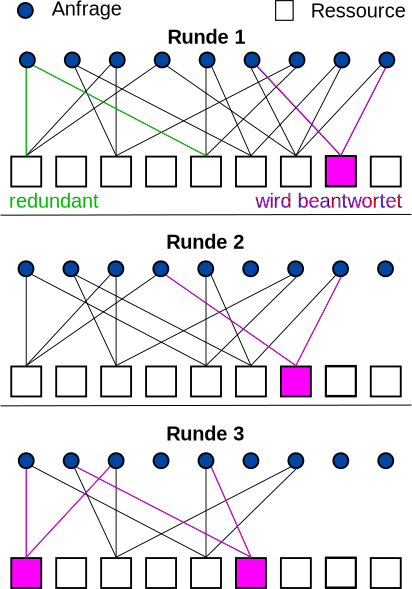
\includegraphics[scale=0.55]{images/ccollision2.pdf}
  \caption{\label{fig:relwork:ccollision} Das $c$-Collision Protokoll: Eine Anfrage wird an alle Ressourcen gestellt, die ein gesuchtes Datum besitzen (grün). Alle Ressourcen, die nach einer Runde höchstens $c=2$ Anfragen haben, beantworten diese (magenta). Alle beantworteten Anfragen werden entfernt.}\phantom{\;\;\;\;\;\;\;\;\;\;\;\;\;\;\;\;\;\;\;\;\;\;}
\end{figure}

In der Arbeit von Petra Berenbrink et al. \cite{ccol2} wird das $c$-Collision Protokoll von Volker Stemann \cite{ccol3} modifiziert, um mit gewichteten Aufgaben arbeiten zu können. Ausgehend von $m$ Bällen, welche auf $n$ Körbe verteilt werden, wird eine untere Schranke für $m \ge n$ ermittelt, in Abhängigkeit der Runden und Anzahl der Körbe. Da jeder Ball ein bestimmtes Gewicht besitzt, wird die Summe über alle Gewichte von Bällen in einem Korb als Last bezeichnet. Außerdem wird ein Zusammenhang zwischen der Anzahl der Bälle, der Gleichförmigkeit ihrer Gewichte sowie der benötigten Laufzeit zur Erreichung einer gegebenen Last untersucht. In dem Algorithmus, dem "`$c$-Load Collision Protocol"', wählt jeder Ball zufällig drei Körbe. Es werden mehrere Runden durchgeführt. In jeder Runde stellt jeder Ball eine Anfrage an alle gewählten Körbe und übermittelt sein Gewicht. Jeder Korb berechnet die Summe der Gewichte von allen Anfragen an ihn. Ist diese Summe höchstens $c$, akzeptiert er, sonst lehnt er ab. Hat ein Ball mindestens eine akzeptierende Antwort bekommen, wird der Ball, samt der durch ihn gestellten Anfragen aus dem Protokoll entfernt.\\
Für das in dieser Arbeit entwickelte System wird ebenfalls der Algorithmus von Berenbrink verwendet (siehe \ref{sec:basics:algos}).
\section{Paralleles Rendering}
\label{sec:relwork:parrender}
Beim parallelen Rendering geht es um digitale Bilderzeugung durch parallele Aufgabenverteilung. Eine populäre Möglichkeit für paralleles Rendering bietet das Scalable Link Interface (SLI), bei dem mehrere Grafikprozessoren zusammengeschlossen werden, um eine höhere Leistung zu erzielen. Es ist aber auch möglich innerhalb eines Netzwerks im Rechnerverbund (Cluster) parallel zu rendern. Dabei wird meist das Rendern selbst in verschiedene Unteraufgaben geteilt. Eine weitere Möglichkeit parallel zu rendern ist die Trennung von Aufgaben, die nichts miteinander zu tun haben, wie zum Beispiel eine Trennung der Datenverwaltung von der Bilderzeugung.\\
In den letzten Jahren wurden viele Möglichkeiten zur Verteilung der Aufgaben in parallelen Rendersystemen veröffentlicht. Steven Molnar et al. \cite{molnar} klassifizieren Parallelisierungsstrategien in drei Kategorien, die sich durch den Ort innerhalb der Rendering-Pipeline unterscheiden, in der die Polygone nach ihrer Sichtbarkeit sortiert werden. Diese drei Kategorien werden Sort-First, Sort-Middle und Sort-Last genannt.

Sort-First-Algorithmen teilen den Bildschirm in Regionen ein (Kacheln) und weisen jedem Renderer eine solche Kachel zu. Jeder Renderer ist für die gesamte Bilderzeugung in diesem einen Bildabschnitt zuständig. Geometrische Objekte werden zu den Renderern übertragen, wenn diese in der jeweiligen Kachel sichtbar sind. Sort-First-Renderer nutzen die Frame-to-Frame-Kohärenz gut aus, da typischerweise nur wenige geometrische Primitive\footnote{Geometrische Primitive sind einfache 3D-Grundkörper (z.B. Kugel, Kegel, Quader, Zylinder, Torus) oder 2D-Grundkörper (z.B. Linie, Kreis, Rechteck, Vieleck, Stern), deren Größe und Grundform über Parameter gesteuert werden können. \cite{medieninfo}} zwischen einzelnen Frames die Bildausschnitte wechseln (Abbildung \ref{fig:relwork:sortfirst}). Die Rendering-Algorithmen sind bei Sort-First frei wählbar, da jeder Renderer die vollständige Geometrie für seine Kachel besitzen muss. Allerdings kann es sein, dass sich viele geometrische Objekte der gesamten Szene auf wenige Kacheln verteilen, wodurch die Lastverteilung aus dem Gleichgewicht gerät. Da jeder Renderer sämtliche geometrischen Primitive innerhalb seiner Kachel zeichnet, werden Objekte redundant bearbeitet, wenn diese von inneren Kachelkanten geschnitten werden.
\begin{figure}
 \centering
  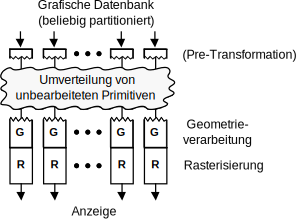
\includegraphics[scale=0.8]{images/sort-first.pdf}
  \caption{Sort-First. Umverteilung von unverarbeiteten Primitiven während der Geometrieverarbeitung. \textit{Quelle: nach \cite{molnar}}}
 \label{fig:relwork:sortfirst}
\end{figure}

Sort-Middle-Algorithmen verteilen hingegen Primitive mitten in der Rendering-Pipeline. Die Trennung erfolgt zwischen der Geometrieverarbeitung und der Rasterisierung. Vor der Verteilung werden die Objekte in screen-space-Koordinaten überführt. Geometrieprozessoren bekommen eine beliebige Untermenge an Primitiven zugewiesen. Rasterisierer bekommen einen Teil des finalen Bildes zugewiesen, ähnlich wie beim Sort-First-Algorithmus. Ob diese beiden Prozessortypen baulich getrennt sind oder ob sie sich einen physikalischen Prozessor teilen, spielt dabei keine Rolle. In der Geometriestufe wird jedes Objekt bezüglich seiner finalen Bildposition klassifiziert und anschließend an die zuständigen Rasterisierer übermittelt (Abbildung \ref{fig:relwork:sortmiddle}). Ein großes Problem bei diesem Verfahren stellt jedoch die Unterbrechung der Rendering-Pipeline dar. In aktuellen Consumer-Grafikkarten ist es entweder sehr teuer, die Pipeline zu unterbrechen, oder es ist überhaupt nicht möglich. Zur Unterbrechung der Rendering-Pipeline müsste die GPU mit der CPU synchronisiert werden, was Zeit kostet und zulasten der Rendering-Bildrate geht.
\begin{figure}
 \centering
  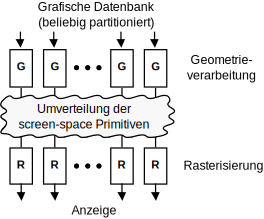
\includegraphics[scale=0.8]{images/sort-middle.pdf}
  \caption{Sort-Middle. Umverteilung von screen-space Primitiven zwischen Geometrieverarbeitung und Rasterisierung. \textit{Quelle: nach \cite{molnar}}}
 \label{fig:relwork:sortmiddle}
\end{figure}

Sort-Last-Algorithmen verteilen geometrische Objekte an einzelne Renderer. Ein Renderer berechnet Pixelwerte für seine Untermenge an Objekten und verteilt die Farb- und Tiefenwerte an Prozesse, die diese dann vereinigen (Abbildung \ref{fig:relwork:sortlast}). Bei großen Objektmengen bietet sich dieses Verfahren an, da jedes geometrische Objekt genau einmal gerendert wird. Für den Pixeltransfer wird allerdings eine hohe Bandbreite im Netzwerk benötigt. Da die genaue Tiefe eines Pixels erst bei der Vereinigung der Pixel ermittelt werden kann, ist Sort-Last für einige Rendertechniken, wie Transparenz oder Antialiasing, schlecht geeignet.
\begin{figure}
 \centering
  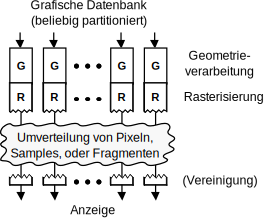
\includegraphics[scale=0.8]{images/sort-last.pdf}
  \caption{Sort-Last. Umverteilung von Pixeln, Samples oder Pixelfragmenten während der Rasterisierung. \textit{Quelle: nach \cite{molnar}}}
 \label{fig:relwork:sortlast}
\end{figure}
Rudrajit Samanta et al. \cite{samanta} haben einen hybriden Renderer entwickelt, welcher Sort-First und Sort-Last-Ansätze kombiniert. Geometrische Objekte werden nach der minimalen Überlappung ihrer Boundingboxen gruppiert und anschließend auf Sort-Last Rechenknoten verteilt. Wird ein Objekt von mehreren Knoten gerendert, weil es deren Kachelgrenzen schneidet, werden die errechneten Tiefenwerte zwischen den betroffenen Knoten ausgetauscht und mit ihren eigenen Tiefenwerten ergänzt. So erhält jeder Renderer ein annähernd korrektes Tiefenabbild. Die fertigen Farbpixel werden am Ende an einen speziellen Kachelrenderer weitergeleitet, welcher lediglich die Kacheln zusammensetzt und darstellt. Der gesamte Pixelversand wird mittels peer-to-peer im Netz\-werk verteilt, wodurch eine verbesserte Netzlastnutzung mit verringerten Latenzen möglich ist.\\
2002 stellten W. V. Baxter et al. \cite{baxter} das parallele Walkthrough-System "`Gigawalk"' vor. Es fasst Objekte zu sogenannten Clustern zusammen. In einem minimalen Spannbaum wird die minimale Ausdehnung eines Clusters berechnet, um mehrere Cluster miteinander verbinden zu können. Eine hierarchische Gruppierung ergibt sich über die Boundingboxen der einzelnen Cluster, woraus ein Szenengraph\footnote{Ein Szenengraph ist eine objektorientierte Datenstruktur, mit der die logische, in vielen Fällen auch die räumliche Anordnung der darzustellenden 2D- oder 3D-Szene beschrieben wird.} erzeugt wird. Aus dieser Hierarchie werden verschiedene Levels-of-Detail (LOD)\cite{hlod} generiert, um bei komplexen Objekten flexibel bleiben zu können. All dies geschieht im Preprocessing. Durch Frustum-Culling werden zur Laufzeit Potentially Visible Sets \cite{RTR3} zusammengestellt, also Mengen an wahrscheinlich sichtbaren Clustern. Um zu verhindern, dass verdeckte Objekte gezeichnet werden, wird ein hierarchischer Z-Buffer verwendet, um ein Occlusion-Culling durchzuführen. Als hierarchische Occluder kommen dabei die berechneten LODs zum Einsatz. Die gesamte Kommunikation erfolgt durch Shared-Memory-Queues. Dieses System wurde mit SGI Onyx Workstations getestet und kommt bei 80 Millionen Dreiecken auf 11-50 Bilder pro Sekunde.\\
Ein anderer Ansatz wird von Ping Yin et al. \cite{DBLP:journals/ijvr/YinJSZ06} verfolgt. Dabei werden Terraindaten berechnet, womit dieses System ohne Occlusion-Culling auskommt, da solche Daten üblicherweise keine große Tiefenkomplexität besitzen. Bemerkenswert bei dieser Arbeit ist, dass die Datenstruktur, ein Quadtree, im Preprocessing erzeugt wird und binär auf Festplatte gespeichert wird. Somit wird ein ständiges Erzeugen einer geeigneten räumlichen Aufteilung des Modells hinfällig. Der Fokus der Arbeit liegt allerdings auf der Kalibrierung des Beamersystems, welches unter Verwendung von Alpha-Blending sichtbare Kanten zwischen einzelnen Displays entfernt.\\
Um der potenziell ungleich verteilten Rendering-Last bei Sort-First-Algorithmen entgegen zu wirken, haben Frederico Abraham et al. \cite{abraham} einen parallelen Renderer entwickelt, der die Kachelgrößen anhand der letzten Renderzeit automatisch anpasst. Jedem Renderknoten im Netzwerk liegt dabei das 3D-Modell vollständig vor. Ein Thread ist immer für die Bilderzeugung zuständig, während ein weiterer sich um den Versand und Empfang von Nachrichten im Netzwerk kümmert. Der Renderknoten, der in einem Frame als erster seine Bildkachel abliefert, bekommt im nächsten Frame die Kachel mit dem höchsten Aufwand zugeteilt. Dieses Kacheltauschen ist jedoch für Out-of-Core Systeme ungeeignet, da die Objektdaten dann ebenfalls umverteilt werden müssen. Außerdem ist ein homogener Rechencluster notwendig, damit Unterschiede in den Rechenzeiten nicht durch unterschiedliche Hardware bedingt sind.

\section{Out-of-Core Rendering}
\label{sec:relwork:oocrender}
Um die höchste Leistung beim Rendering erzielen zu können, sollte sich eine 3D-Szene vollständig im schnellen Speicher der Grafikkarte befinden. Komplexität und Größe der 3D-Modelle steigt proportional zur Grafikspeicherkapazität, weshalb Teile von komplexen 3D-Modellen in den Hauptspeicher ausgelagert werden müssen. Doch auch der ist begrenzt. Von Out-of-Core Rendering wird gesprochen, wenn ein zu renderndes 3D-Modell nicht vollständig im Arbeitsspeicher vorliegt. Man könnte kleinere Mengen des Modells einzeln rendern und am Ende die Bilder vereinigen. Das resultierende Bild ist so zwar fehlerfrei, allerdings geht dieses Verfahren zulasten der Rendergeschwindigkeit. Eine weitere Möglichkeit besteht darin, Teile des Modells wegzulassen, bis der verbleibende Rest nicht mehr zu groß für den Grafik- oder Hauptspeicher ist. In einigen Fällen wird dies auch gemacht, es führt jedoch zu Bildfehlern, da Teile fehlen können, die eigentlich sichtbar sind.

Dinesh Manocha und Gokul Varadhan \cite{manocha} stellen ein Out-of-Core System vor, mit dem sich interaktive Bildraten in einem Verbund mehrerer SGI Workstations erzielen lassen. Durch den Einsatz mehrerer Rechner ist dieses Verfahren kein reines Out-Of-Core System, da es auch parallel arbeitet. Ein Prefetching-Thread versucht Objekte im Voraus zu laden, wodurch Popping-Artefakte reduziert werden. In Rendering-Systemen gibt es virtuelle Kameras um die Bilderzeugung zu steuern,  welche ähnlichen Eigenschaften wie tatsächliche Kameras besitzen. Durch Erweiterung des eigentlichen View-Frustums verhält sich die Kamera in Manochas System ähnlich wie bei einem Weitwinkelobjektiv. Durch diese Technik werden Objekte an den Rändern schon geladen, obwohl sie noch nicht sichtbar sind. Sollten sie in einem nachfolgenden Frame benötigt werden, sind sie dadurch sofort einsetzbar. Zusätzlich werden beim Prefetching Objekte, die nur im erweiterten Frustum liegen, durch den Winkel zum Zentrum der Kamera priorisiert, wodurch Objekte, welche näher am Kamerazentrum liegen, bevorzugt werden. Wie viel größer das erweiterte Frustum ist, hängt von der aktuellen Bewegungsgeschwindigkeit ab.\\
Auch Wagner T. Corr\^{e}a et al. \cite{wagner1}, \cite{wagner2} speichern eine hierarchische Repräsentation des Modells in einem Preprocessing-Schritt auf der Festplatte ab. Ihr System ist eine parallele Erweiterung ihres eigenen iWalk-Renderers \cite{iwalk}. Mit dieser Erweiterung sind sie in der Lage, Bilder mit sehr hohen Auflösungen (4096$\times$3072 Pixel) zu erstellen. Das System arbeitet in einem Rechencluster von 16 Pentium4-PCs mit je 512MB RAM. Jeder Rechenknoten besitzt ein festgelegtes Kontingent an Dreiecken und Speicherverbrauch. Unter Einhaltung dieses Kontingents wird für jeden Frame die sichtbare Geometrie in Form von Octree-Knoten über Prioritized-Layered Projections (PLP) \cite{plp} bestimmt. Ein Vorteil von PLP besteht darin, dass eine hierarchische Struktur des Modells während des Preprocessings erzeugt werden kann. Dadurch können die sichtbaren Octree-Knoten zur Laufzeit bestimmt werden, ohne dabei auf die tatsächliche Szenengeometrie zugreifen zu müssen. Es gibt einen separaten Caching-Thread, der Objekte eine Weile im Speicher belässt und das Prefetching organisiert. Objektanfragen den aktuellen Frame betreffend werden dabei jedoch bevorzugt. Als Verdrängungsstrategie kommt Least-Recently-Used (LRU) zum Einsatz.\\
Bei Ingo Wald et al. \cite{wald} wird das Modell der Boeing 777 mit einem Raytracing-Verfahren gerendert. Dieses Modell wird auch in der vorliegenden Arbeit verwendet. Hierbei wird die gesamte Boeing auf einem Dual-Core 1.8GHz Opteron-PC mit 6GB RAM gerendert. Die Speicherverwaltung arbeitet mittels Memory-Mapped-I/O, womit Teile der Festplatte direkt in den Arbeitsspeicher gespiegelt werden können. Da ständiges Ein- und Auslagern der Speicherseiten viel Zeit kostet, hat man sich entschieden, eine solche Verwaltung für den Raytracer selbst zu entwickeln. Im Vorfeld werden sogenannte Geometrie-Proxies erstellt, die wegen ihrer geringen Größe vollständig im Speicher des Renderers abgelegt werden. Wird ein Modellteil benötigt, so ist die Speicheradresse an der es sich befinden müsste, bekannt. Ist es vorhanden, wird es gerendert, ansonsten wird aus einer Hash-Map über die Adresse der entsprechende Proxy gerendert. Mit entsprechenden Systemaufrufen können Speicherseiten direkt ausgelagert werden oder länger als üblich aktiv im Speicher gehalten werden. Durch dieses System wurden bei einer Auflösung von 640$\times$480 Pixeln 3-7 Bilder pro Sekunde erreicht.

% EOF
%

\chapter{Grundlagen}
\label{chap:basics}
\todo[size=\small, inline]{Evtl. besseren Namen für Kapitel "`Grundlagen"' finden $\rightarrow$ Grundlegende Algorithmen/Techniken?!}%
\textbf{Hier kommt nur rein was ICH mache!}\\
An dieser Stelle soll zunächst ein Überblick über die in der vorliegenden Arbeit verwendeten Techniken gegeben werden. Diese beinhalten unter anderem Algorithmen der Computergrafik, welche Datenstrukturen benutzt werden und wie die Speicherverwaltung organisiert ist.

\section{Datenstrukturen}
\label{sec:basics:datenstrukturen}
\textbf{Wofür und warum?!}\\
3D-Modelle aus Computer Aided Design - Anwendungen (CAD) werden üblicherweise nach ihrer Funktion gruppiert. Das mag beim Entwurf solcher Systeme auch praktisch sein, bei der Visualisierung kann dies jedoch zu Problemen führen. Bei CAD-Modellen in Größenordnung der Boeing 777\footnote{\todo[size=\small, inline]{Boeing Herkunftshinweis verschieben an die erste Stelle wo es erwähnt wird.}%
Das 3D-Modell der Boeing 777 wurde freundlicherweise zur Verfügung gestellt von The Boeing Company, Seattle, WA, USA.} (ca. 350 Millionen Dreiecke) ist es wichtig, dass diese in eine geeignete räumliche Unterteilung überführt werden. Da ein Out-Of-Core-Renderer entwickelt wurde, findet ein ständiges Laden und Verwerfen von Teilmodellen statt. Je länger ein Renderer benötigt um herauszufinden, welche Teile des Modells er verwerfen kann und welche er als erstes anfordern sollte, desto länger braucht er auch um ein Bild zu erstellen. In dieser Arbeit wurde als hierarchische räumliche Unterteilung ein Randomized Sampletree (\ref{sec:basics:sampletree}) und zum Vergleich ein Loose Octree gewählt.

\subsection{Loose Octree}
\label{sec:basics:octree}
Um einen Octree \cite{RTR3} zu Erzeugen wird die gesamte Szene in eine minimale Boundingbox eingeschlossen. Rekursiv wird diese Box entlang der drei räumlichen Achsen in der Mitte geteilt, woraus sich jeweils acht gleich-große Boundingboxen ergeben. Dieser Vorgang wird so lange wiederholt bis ein Haltekriterium erfüllt ist. Im Falle der Boeing wurde festgelegt, dass höchstens 5.000 Dreiecke in einer Box liegen dürfen und die maximale Tiefe des Baums wurde auf 14 beschränkt. Erfüllt ein Octree-Knoten eines dieser Kriterien, wird nicht weiter untereilt. Dementsprechend gibt es keine leeren Blatt-Knoten im Octree. In Abbildung \ref{fig:basics:octree} ist ein Octree zu sehen.\\
\begin{figure}
 \centering
  \includegraphics[scale=0.5]{images/octree.pdf}
 % octree.pdf: 640x368 pixel, 72dpi, 22.58x12.98 cm, bb=0 0 640 368
  \caption{Ein Octree der Tiefe 2. \textit{links: die räumliche Darstellung, rechts: die Baumdarstellung. Quelle: \htmladdnormallink{http://de.wikipedia.org/wiki/Octree}{http://de.wikipedia.org/wiki/Octree}}}
 \label{fig:basics:octree}
\end{figure}
In dieser Arbeit wurde jedoch eine spezielle Form des Octrees verwendet: der Loose Octree. Dieser erweitert den Octree um eine weitere Box pro Knoten: die sogenannte Loosebox. Sie teilt sich ihr Zentrum mit der Octree-Boundingbox, besitzt aber doppelte Kantenlängen. Wird nun festgestellt, dass in einem Knoten mehr als 5.000 Dreiecke liegen, wird die größe der einzelnen Dreiecke anhand der Loosebox geprüft. Liegt ein Dreieck vollständig in der Loosebox mit seinem Zentrum in der eigentlichen Boundingbox des Knotens, kann es weiter nach unten gereicht werden. Ist dies nicht der Fall, ist das Dreieck zu groß für den aktuellen Knoten und wird an den Vaterknoten gegeben (Abbildung \ref{fig:basics:looseoctree}).\\
Dies hat den Vorteil, dass große Dreiecke relativ weit oben im Baum zu liegen kommen und Kleinere entsprechend tief. Je größer ein Dreieck ist, desto größer ist auch die Wahrscheinlichkeit, dass das Dreieck sichtbar ist und somit gezeichnet werden muss. Bewegt man sich durch ein Modell, ist der Wurzelknoten, oder Szenen-Boundingbox, praktisch immer sichtbar, was bedeutet, dass die zur Wurzel gehörige Geometrie gezeichnet werden muss.
\begin{figure}
 \centering
  \includegraphics[scale=0.8]{images/looseoctree2.pdf}
  \caption{Ein Loose Octree in einer 2D-Darstellung. \textit{Das Zentrum des Objekts (rosa) befindet sich innerhalb der Octree Zelle, das gesamte Objekt befindet sich innerhalb der Loose Box. Quelle: \htmladdnormallink{http://anteru.net/2008/11/14/315/}{http://anteru.net/2008/11/14/315/}}}
 \label{fig:basics:looseoctree}
\end{figure}

\subsection{Randomized Sampletree}
\label{sec:basics:sampletree}
Als spezielle Ausprägung eines Loose Octrees gibt es den Randomized Sampletree \cite{klein}. Dieser unterschiedet sich von einem Octree darin, dass zufällig einzelne Dreiecke aus tieferen Knoten in höhere Knoten verschoben  wurden. Beim rendern der Szene wird in jedem Frame der Baum traversiert, um ein Frustum-Culling durchzuführen (siehe auch \ref{sec:basics:algos:frustumculling}). Ab einer bestimmten Tiefe im Baum wird die Traversion abgebrochen, um die Komplexität der Darstellung zu reduzieren. Dadurch kommt es allerdings zu Darstellungsfehlern, da nicht alle sichtbare Geometrie gerendert wird. An dieser Stelle schafft ein Randomized Sampletree abhilfe. Dadurch dass zufällige kleinere Dreiecke in höherliegenden Knoten gespeichert sind, werden diese auch gerendert. Ist die Flächensumme alle Dreiecke in einem Knoten des Sampletrees nicht größer als ein Pixel, wird die Traversion abgebrochen. Klein, Krokowski und Fischer \cite{klein} haben gezeigt, dass diese Geometrie-Approximation von weit entfernten Objekten durch zufällige Dreiecke eine hinreichend korrekte Darstellung liefert. Dieses Verfahren wurde für komplexe geometrische Umgebungen entwickelt, weshalb es in dieser Arbeit verwendet wurde.
\begin{figure}
 \centering
  \includegraphics[scale=1.7]{images/sampletree2.pdf}
  \caption{Ein Sampletree in einer 2D-Darstellung. \textit{links: Eine Aufteilung von Polygonen in verschiedene Quadtree Zellen. rechts: Die Baumdarstellung des Sampletrees. Die farbigen Knoten geben an welche Polygonteile der linken Seite in welchen Knoten gespeichert wurden. Quelle: \cite{klein}}}
 \label{fig:basics:sampletree}
\end{figure}

\section{Computergrafik}
\label{sec:basics:computergrafik}
\todo[size=\small, inline, color=yellow]{Computergrafik $\rightarrow$ Spellcheck!}
Da Arbeitsspeicher in der Regel größer ist als der Speicher einer Grafikkarte, werden nicht alle geometrischen Objeke auf der Grafikkarte belassen. Wenn angeforderte Objekte bei einem Renderer eintreffen, werden die zunächst gar nicht an die Grafikkarte geschickt. Erst nach weiteren Tests, ob das Objekt immer noch sichtbar ist, findet der transfer zur GPU statt. Dort verbleiben sie dann, bis sie irgendwann aus platz- oder sichbarkeitsgründen verdrängt werden (siehe auch \ref{sec:basics:caching}). Um dies möglichst effizient umsetzen zu können werden Vertexbuffer Objects  (VBOs) genutzt. Die Idee ist dabei, dass Modelldaten, bestehend aus Vertices und Vertex-Normalen, in einem zusammenhängenden Speicherblock abgelegt werden. Ein Vertex besteht aus einer $xyz$-Koordinate und einer Vertex-Normalen. Der Zugriff auf Dreiecke erfolgt dann mittels einer Index-Liste, bei der immer drei Indices ein Dreieck ergeben. Alle Dreiecke eines Octree-Knotens wurden zu einem Vertexbuffer-Objekt zusammen gefasst (siehe \ref{sec:basics:octree}), da Geometrie innerhalb eines Knotens nicht weiter unterteilt wird. In Form von VBOs kann recht einfach entsprechender Platz im Grafik-RAM reserviert und die Daten in den Speicher geladen werden.\\
Im Gegensatz dazu verbleiben bei Vertex-Arrays alle Daten im Arbeitsspeicher des Rechners und werden für jeden Zeichenaufruf zur Grafikkarte übertragen. Vertex-Arrays bieten sich an, wenn Objekte nur einmal gezeichnet und dann verworfen werden. Von daher kommen sie nur auf den Datenknoten (siehe \ref{sec:impl:netzwerkarchitektur}) zum Einsatz, da diese ein getestetes Objekt nur in ihren Tiefenbuffer rendern und dann wieder verwerfen. Bei VBOs wäre der Overhead der Datenübertragung und der anschließenden Deallokation zu groß für eine einmalige Verwendung.

Das Modell der Boeing 777 besitzt auch Farbinformationen. Da bei CAD-Modellen Farben oft einen Hinweis auf den Produktionsort geben, ist die Anzahl der Farben beschränkt. Natürlich könnte man jedem Vertex eine Farbe zuordnen. Dies hätte jedoch zur Folge dass bei jedem Vertex die Farbe neu gesetzt werden muss, unabhängig davon, ob diese Farbe bereits gesetzt ist. Das würde jedesmal die Grafik-Pipeline unterbrechen und es wäre mit Geschwindigkeitseinbußen zu rechen. Deshalb wurden die Farben der Boeing, 32 an der Zahl, in einer 1D-Textur kodiert und die Texturkoordinate wurde als vierte Komponente an den Vertex gehängt. Wird nun ein Vertex gezeichnet, ersetzt der Vertex-Shader die harmonische vierte Komponente eines Vertices wieder durch $1.0$ und gibt die Textur-Koordinate an den Fragment-Shader weiter. Letzterer muss ohnehin eine Farbe schreiben, weshalb diese kurzerhand aus der Textur ausgelesen wird. Da die Anzahl der Farben bekannt ist ist, ergibt sich zur Berechnung der Texturkorrdinate der $i$-ten Farbe $\frac{i}{n}-\frac{1}{2n}$, wobei $n=$  Anzahl der Farben ist (Abbildung \ref{fig:basics:1dtexture}). Die Subtraktion der Hälfte eines Texels $\frac{1}{2n}$ ist Notwendig, da man sonst genau auf der Kante zwischen zwei Farben landet, was zu undefiniertem Farbverhalten in der Grafikkarte führt.
\begin{figure}
  \centering
  %%%%%%%%%%%%%%%%%%%%%%%%%%%%%%%%%%%%%%%%%%%%%%%%%%%%%%%%%
% 1D-Farbtextur mit Beschreibung und Labels
%%%%%%%%%%%%%%%%%%%%%%%%%%%%%%%%%%%%%%%%%%%%%%%%%%%%%%%%%


\begin{tikzpicture}
  \tikzset{ 
    every pin/.style={fill=yellow!50!white,rectangle,rounded corners=3pt,font=\tiny}, 
    small dot/.style={fill=black,circle,scale=0.3} } 
  \begin{axis}[
    x=10cm, y=0.5cm, 
    clip=false,
    ytick=\empty,
    xtick={0,0.03125,0.0625,0.09375,0.125,0.15625,0.1875,0.21875,0.25,0.28125,0.3125,
      0.34375,0.375,0.40625,0.4375,0.46875,0.5,0.53125,0.5625,0.59375,0.625,
      0.65625,0.6875,0.71875,0.75,0.78125,0.8125,0.84375,0.875,0.90625,0.9375,
      0.96875,1},
    xticklabels={$0$,$\frac{1}{n}$,$\frac{2}{n}$,$\frac{3}{n}$,$\frac{4}{n}$,$\frac{5}{n}$,$\frac{6}{n}$,$\frac{7}{n}$,$\frac{8}{n}$,$\frac{9}{n}$,$\frac{10}{n}$,
      $\frac{11}{n}$,$\frac{12}{n}$,$\frac{13}{n}$,$\frac{14}{n}$,$\frac{15}{n}$,$\frac{16}{n}$,$\frac{17}{n}$,$\frac{18}{n}$,$\frac{19}{n}$,$\frac{20}{n}$,
      $\frac{21}{n}$,$\frac{22}{n}$,$\frac{23}{n}$,$\frac{24}{n}$,$\frac{25}{n}$,$\frac{26}{n}$,$\frac{27}{n}$,$\frac{28}{n}$,$\frac{29}{n}$,$\frac{30}{n}$,
      $\frac{31}{n}$,$\frac{32}{n}$},
    tick label style={
    font=\tiny},
    %major x tick num=5,
    %hide y axis,
    enlargelimits=false,
    axis on top] 
    \addplot graphics [xmin=0,xmax=1,ymin=0,ymax=1, 
      % trim=left bottom right top 
      includegraphics={trim=0 9 0 8,clip}
      ] 
      {images/1d_texture.pdf}; 

\node[small dot,pin=-90:{$\frac{1}{2n}$}] at (axis description cs:0.017625,0) {}; 
%\node[small dot,pin=-45:{$\frac{1}{n}$}] at (axis description cs: 0.03325,0) {}; 

  \end{axis} 
\end{tikzpicture}
  \caption{1D-Farbtextur. $n=$Anzahl Farben. Um mittig auf den Texel der Farbe $i$ zuzugreifen, errechnet sich die Texturkoordinate durch $\frac{i}{n}-\frac{1}{2n}$. }
  \label{fig:basics:1dtexture}
\end{figure}

\section{Algorithmen}
\label{sec:basics:algos}
\todo[size=\small, inline, color=magenta]{Kapitel: Algorithmen}
\begin{itemize}
  \item Intro
\end{itemize}

\begin{figure}
  \centering
  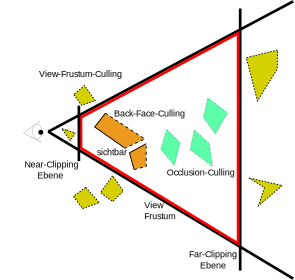
\includegraphics[scale=0.8]{images/culling.pdf}
  \caption{Verschiedene Culling-Techniken. Entfernte Geometrie ist durch gestrichelte Linien dargestellt. \textit{Quelle: \cite{culling}} }
  \label{fig:basics:culling}
\end{figure}
\begin{itemize}
  \item Culling \cite{RTR3}\label{sec:basics:algos:culling}
  \begin{itemize}
    \item entfernen von Szenenteilen die nicht zum finalen Bild beitragen (Abbildung \ref{fig:basics:culling})
    \item In jeder Renderstufe möglich.
    \item einige Algos sind in Hardware implementiert. Für volle Kontrolle kann aber auch alles auf der CPU gemacht werden.
    \item Davon ausgehend, dass sich der Flaschenhals nicht auf der CPU befindet, the fastest polygon to render is the one never sent down the accelerator's pipeline.
    \item Der Ideale Culling-Algo würde nur die \textit{exakte sichtbare Menge} an Primitiven durch die Pipeline schicken. Erzeugen solcher Datenstrukturen ist theoretisch möglich, aber nicht praktikabel, da die worst-case Zeitkomplexität $O(n^{9})$ \cite{culling} beträgt.
    \item Stattdessen wird versucht die \textit{potentiell sichtbare Menge} (Potentially Visible Set)[PVS] zu finden. Ist in einem PVS die exakt sichtbare Menge nicht vollständig enthalten, wird das Verfahren als \textit{approximativ} bezeichnet. Diese Art von PVS kann zu fehlerhalften Bildern führen.
  \end{itemize}
  \item Backface Culling
  \begin{itemize}
    \item entfernen von poygonen welche vom Betrachter abgewandt sind
    \item wird jeweils auf einzelnen Polygonen durchgeführt
    \item Wird bei uns von der API (Hardware/OpenGL) durchgeführt
  \end{itemize}
  \todo[size=\small, inline]{Stichwortliste aus dem Buch vervollständigen.}
  \item View-Frustum Culling \cite{RTR3} \label{sec:basics:algos:frustumculling}
  \begin{itemize}
    \item Entfernt Polygongruppen, die sich außerhalb des View-Frustums befinden.
  \end{itemize}
  \item Occlusion Culling \cite{RTR3}\label{sec:basics:algos:occlusionculling}
  \begin{itemize}
    \item Entfernt Polygone die durch andere andere Polygongruppen verdeckt sind
  \end{itemize}
  \item $c$-Collision Protokoll zur Lastbalancierung im Netzwerk \label{sec:basics:algos:ccollision} (siehe \ref{chap:relwork})
  \item dynamische Kachelung
  \item (extended Frustum?)
\end{itemize}

\subsection{Caching}
\label{sec:basics:caching}
\todo[size=\small, inline, color=blue!40]{Kapitel: Caching}
\begin{itemize}
 \item wird über Algos gefüllt
\end{itemize}

\subsection{Speichermanagement}
\label{sec:basics:speichermanagement}
\todo[size=\small, inline, color=blue!40]{Kapitel: Speichermanagement}
\begin{itemize}
 \item nicht jeder braucht alles -> Kacheln
 \item Gewichtung über die Anzahl der Dreiecke pro Request
\end{itemize}

\section{Approximation}
\label{sec:basics:approximation}
\todo[size=\small, inline, color=blue!40]{Unterkapitel: Approximation}
Approximationen in der Computergrafik haben oft  Zurfolge, dass die Bildqualität verringert wird. Sei es weil Objekte in niedrigeren Auflösungen
\begin{itemize}
 \item Occlusion-Culling entfernt teile
 \item Nicht immer sofort ein vollständiges Bild verfügbar -> nach und nach nachladen
 \item Teile können weggelassen werden $\rightarrow$ OcclusionCulling \& FrustumCulling
 \item Begrenzung des Cache-Kontingents
 \item Tiefenbuffer Update nur alle paar Frames
 \item Sampletree
\end{itemize}


\chapter{Implementierung}
\label{impl}
Kapiteleinleitung\\*
Ankündigung des Bedarfs an günstigen Approximationen für Backend-Knoten -> Verweis auf Clemens\\
C++, OpenGL, STL, usw.
Probleme / Herausforderungen in die Unterpunkte ziehen
\begin{itemize}
 \item Speicherverwaltung
 \item Preprozessing
 \item From Scratch entwickelt / keine Erweiterung eines bestehenden Systems
 \item Filesystem
\end{itemize}
\section{Preprocessing}
\label{impl:preprocessing}
Aufbereitung der Model-Daten in ein verständliches Format
\section{Datenstruktur}
\label{impl:datenstruktur}
Verewigt auf HDD -> begründen warum
\section{Netzwerkarchitektur}
\label{impl:netzwerkarchitektur}
Hardwarebeschaffenheit und die NodeTypen
\section{Kommunikation}
\label{impl:kommunikation}
Sequenzdiagramm
\begin{figure}
 \centering
  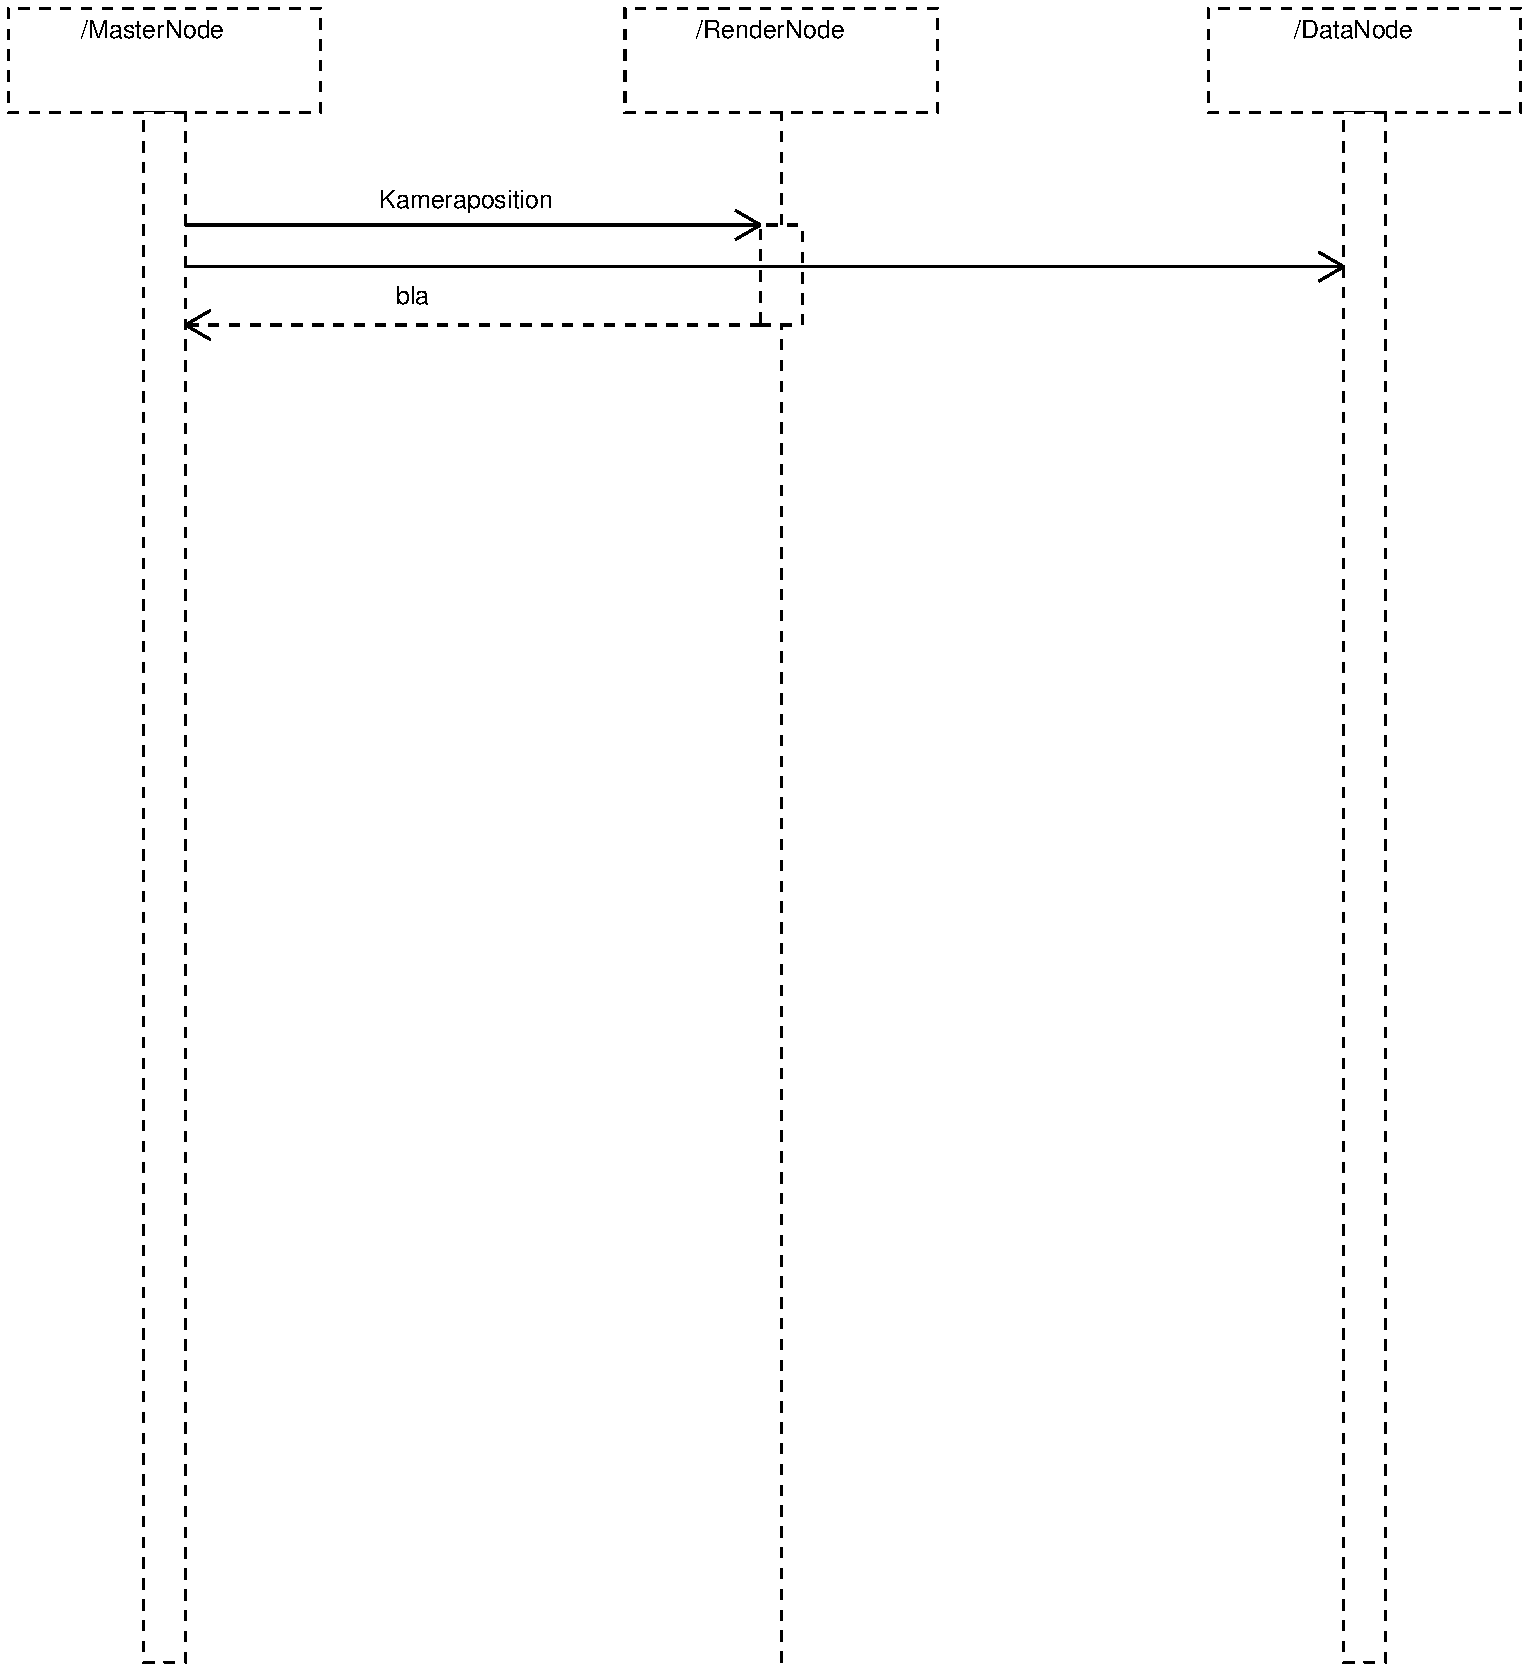
\includegraphics[scale=0.5]{images/Sequenzdiagramm.pdf}
  % Sequenzdiagramm.pdf: 1358x804 pixel, 72dpi, 47.91x28.36 cm, bb=0 0 1358 804
  \caption{Ein Sequenzdiagramm}
 \label{fig:seqdiag}
\end{figure}

\begin{center}
\end{center}

\section{Rendering-Algorithmus}
\label{impl:renderalgo}
\begin{itemize}
 \item wie wird gerendert?
 \item wo kriegen die ihre Daten her?
 \item wird die Last balanciert
\end{itemize}


%
% EOF
%

\chapter{Evaluierung}
\todo[size=\small, color=blue!40, inline]{Kapitel: Evaluierung}%
\begin{itemize}
 \item wie skaliert das System / bringt es was?
 \item Cache löschen - neu laden -> Zeit messen
 \item Verschiedene Kamerapositionen:
 \begin{itemize}
  \item Turbine
  \item Cockpit
  \item Heck
  \item ``Businessclass''
  \item seitlich von Außen
 \end{itemize}
 \item Erklärung der Tests \& Diagramme
 \item Balancierung durch c-Collision Protokoll / die Varianz
\end{itemize}




%  ----------------------------------------------------------------------------
%
%       Copyright (for the thesis) 2009 by [author - insert yourself]
%
%       This thesis is published under the
%       Creative Commons Attribution-No Derivative Works 3.0 Austria License
%       as detailed at http://creativecommons.org/licenses/by-nd/3.0/at/
%
%  ----------------------------------------------------------------------------
%  Template credits and license:
%  ----------------------------------------------------------------------------
%
%       "Fakultät für Informatik" diploma/master thesis template 2008
%
%       based upon "Diploma thesis template 2005" by lukas.silberbauer(at)gmx.at
%       based upon "Diplomarbeit mit LaTeX" by Tobias Erbsland
%       incorporating a title page by Informatik-Forum user "Baby"
%       polished and ported to the TU fonts package by Jakob Petsovits
%
%       published under the terms of
%
%  ----------------------------------------------------------------------------
%  "THE BEER-WARE LICENSE":
%  <lukas.silberbauer(at)gmx.at> wrote this file. As long as you retain this
%  notice you can do whatever you want with this stuff. If we meet some day,
%  and you think this stuff is worth it, you can buy me (us) a beer in return.
%  ----------------------------------------------------------------------------
%
%  (end of template credits)
%

\chapter{Fazit und Ausblick}
\label{conclusion}

Ausblick:
\begin{itemize}
 \item Mechanismen zur Bildkompression verwenden bevor RGB- oder Tiefen-Informationen verschickt werden.
  \item Ankündigung des Bedarfs an günstigen Approximationen für Backend-Knoten $\rightarrow$ Verweis auf Clemens
\end{itemize}

%
% EOF
%




\appendix

\bibliographystyle{unsrtdin}
\bibliography{bib/references}

\listoffigures

%\addcontentsline{toc}{chapter}{Abbildungsverzeichnis}
%\listoftables
%\listofalgorithms
%\addcontentsline{toc}{chapter}{Tabellenverzeichnis}

%  ----------------------------------------------------------------------------
%
%       Copyright (for the thesis) 2009 by [author - insert yourself]
%
%       This thesis is published under the
%       Creative Commons Attribution-No Derivative Works 3.0 Austria License
%       as detailed at http://creativecommons.org/licenses/by-nd/3.0/at/
%
%  ----------------------------------------------------------------------------
%  Template credits and license:
%  ----------------------------------------------------------------------------
%
%       "Fakultät für Informatik" diploma/master thesis template 2008
%
%       based upon "Diploma thesis template 2005" by lukas.silberbauer(at)gmx.at
%       based upon "Diplomarbeit mit LaTeX" by Tobias Erbsland
%       incorporating a title page by Informatik-Forum user "Baby"
%       polished and ported to the TU fonts package by Jakob Petsovits
%
%       published under the terms of
%
%  ----------------------------------------------------------------------------
%  "THE BEER-WARE LICENSE":
%  <lukas.silberbauer(at)gmx.at> wrote this file. As long as you retain this
%  notice you can do whatever you want with this stuff. If we meet some day,
%  and you think this stuff is worth it, you can buy me (us) a beer in return.
%  ----------------------------------------------------------------------------
%
%  (end of template credits)
%

\chapter{Glossar}

\begin{acronym}
\acro{API}{Application Programming Interface}
\acro{CAD}{Computer Aided Design}
\acro{CPU}{Central Processing Unit (Hauptprozessor)}
\acro{FPS}{Frames per second}
\acro{GPU}{Graphics Processing Unit (Grafikprozessor)}
\acro{HLOD}{Hierarchical Level-Of-Detail\mycite{hlod}}
\acro{KD-Baum}{Ein k-dimensionaler Baum oder KD-Baum ist ein unbalancierter Suchbaum zur Speicherung von Punkten. (siehe\mycite{RTR3}, Seite 650 ff.)}
\acro{LOD}{Level-Of-Detail (siehe\mycite{RTR3}, Seite 680 ff.)}
\acro{PLP}{Prioritized-Layered Projection\mycite{plp}}
\acro{Octree}{Ein Octree ist eine räumliche Datenstruktur, bestehend aus einem gewurzelten Baum, dessen Knoten jeweils entweder acht direkte Nachfolger oder gar keine Nachfolger haben.}
\acro{peer-to-peer}{Peer-to-peer Netzwerke sind Netzwerksysteme ohne zentrale Zugriffskontrolle, in denen alle Rechner gleichberechtigt agieren. Eine Datenverbindung besteht dabei immer direkt von einem Teilnehmer zum anderen.}
\acro{PVS}{Potentially Visible Set (siehe\mycite{RTR3}, Seite 660 ff.)}
\acro{Quantil}{Ein $p$-Quantil ist ein Lagemaß in der Statistik, wobei $p$ eine reelle Zahl zwischen 0 und 1 ist. Das $p$-Quantil ist ein Merkmalswert, der die Verteilung einer Variablen bzw. Zufallsvariablen in zwei Teile teilt. Links vom $p$-Quantil liegen $100\cdot p$ Prozent aller Beobachtungswerte bzw. $100\cdot p$ Prozent der Masse der Zufallsvariablen. Rechts davon liegen $100\cdot(1-p)$ Prozent aller Beobachtungswerte bzw. $100\cdot(1-p)$ Prozent der Masse der Zufallsvariablen.}
\acro{Quartil}{Quartile sind die Quantile 0,25-Quantil, 0,5-Quantil=Median und 0,75-Quantil.}
\acro{Rasterisierung}{Überführung eines kontinuierlichen Raums in einen diskreten Raum (Pixel).}
\acro{Rendering}{Erzeugt ein 2D-Bild aus einer 3D-Szene.}
\acro{Textel}{Texturelement}
\acro{screen-space}{Projektion einer 3D-Szene in einen zweidimensionalen Raum (Bild).}
\acro{SGI}{SGI ist ein Hersteller von Computern, die besonders auf dem Gebiet der grafischen Darstellung leistungsstark sind (Grafik-Workstation).}
\acro{SLI}{Scalable Link Interface; Zusammenschluss mehrer Grafikchips}
\acro{View-Frustum}{Sichtfeld der Kamera}
\end{acronym}

%
% EOF
%

%  ----------------------------------------------------------------------------
%
%       Copyright (for the thesis) 2009 by [author - insert yourself]
%
%       This thesis is published under the
%       Creative Commons Attribution-No Derivative Works 3.0 Austria License
%       as detailed at http://creativecommons.org/licenses/by-nd/3.0/at/
%
%  ----------------------------------------------------------------------------
%  Template credits and license:
%  ----------------------------------------------------------------------------
%
%       "Fakultät für Informatik" diploma/master thesis template 2008
%
%       based upon "Diploma thesis template 2005" by lukas.silberbauer(at)gmx.at
%       based upon "Diplomarbeit mit LaTeX" by Tobias Erbsland
%       incorporating a title page by Informatik-Forum user "Baby"
%       polished and ported to the TU fonts package by Jakob Petsovits
%
%       published under the terms of
%
%  ----------------------------------------------------------------------------
%  "THE BEER-WARE LICENSE":
%  <lukas.silberbauer(at)gmx.at> wrote this file. As long as you retain this
%  notice you can do whatever you want with this stuff. If we meet some day,
%  and you think this stuff is worth it, you can buy me (us) a beer in return.
%  ----------------------------------------------------------------------------
%
%  (end of template credits)
%

\chapter{Zusätzliche Abbildungen}
\label{chap:add_fig}

\begin{Bild}
\includegraphics[scale=0.40]{images/pos1.pdf}
\captionof{figure}{\label{fig:eval:pos1}Kameraposition 1 \textit{(Heck außen, 3.352.475 sichtbare Dreiecke)}}
\end{Bild}

\begin{Bild}
\includegraphics[scale=0.40]{images/pos2.pdf}
\captionof{figure}{\label{fig:eval:pos2}Kameraposition 2 \textit{(Heck innen, 2.045.104 sichtbare Dreiecke)}}
\end{Bild}

\begin{Bild}
\includegraphics[scale=0.40]{images/pos3.pdf}
\captionof{figure}{\label{fig:eval:pos3}Kameraposition 3 \textit{(Passagierbereich, 3.749.977 sichtbare Dreiecke)}}
\end{Bild}

\begin{Bild}
\includegraphics[scale=0.40]{images/pos4.pdf}
\captionof{figure}{\label{fig:eval:pos4}Kameraposition 4 \textit{(Stauraum, 8.381.277 sichtbare Dreiecke)}}
\end{Bild}

\begin{Bild}
\includegraphics[scale=0.40]{images/pos5.pdf}
\captionof{figure}{\label{fig:eval:pos5}Kameraposition 5 \textit{(Fahrwerk/Flügel, 5.776.159 sichtbare Dreiecke)}}
\end{Bild}

\begin{Bild}

\includegraphics[scale=0.40]{images/pos6.pdf}
\captionof{figure}{\label{fig:eval:pos6}Kameraposition 6 \textit{(Turbine, 3.381.998 sichtbare Dreiecke)}}
\end{Bild}

\begin{Bild}

\includegraphics[scale=0.40]{images/pos7.pdf}
\captionof{figure}{\label{fig:eval:pos7}Kameraposition 7 \textit{(Nase innen, 1.481.706 sichtbare Dreiecke)}}
\end{Bild}

\begin{Bild}

\includegraphics[scale=0.40]{images/pos8.pdf}
\captionof{figure}{\label{fig:eval:pos8}Kameraposition 8 \textit{(Cockpit, 4.558.623 sichtbare Dreiecke)}}
\end{Bild}

\begin{Bild}

\includegraphics[scale=0.40]{images/pos9.pdf}
\captionof{figure}{\label{fig:eval:pos9}Kameraposition 9 \textit{(Nase außen, 7.439.695 sichtbare Dreiecke)}}
\end{Bild}

\begin{Bild}

\includegraphics[scale=0.40]{images/pos10.pdf}
\captionof{figure}{\label{fig:eval:pos10}Kameraposition 10 \textit{(Flügel-Rumpf Bereich, 4.066.296 sichtbare Dreiecke)}}
\end{Bild}

\begin{Bild}
\includegraphics[scale=0.40]{images/button.pdf}
\captionof{figure}{\label{fig:eval:button}Türknopf \textit{(Bug)}}
\end{Bild}

\begin{Bild}
\includegraphics[scale=0.40]{images/profil_bug.pdf}
\captionof{figure}{\label{fig:eval:prof_bug}Profil \textit{(Bug)}}
\end{Bild}

\begin{Bild}
\includegraphics[scale=0.40]{images/profil_heck.pdf}
\captionof{figure}{\label{fig:eval:prof_heck}Profil \textit{(Heck)}}
\end{Bild}

\begin{Bild}
\includegraphics[scale=0.40]{images/turbine_innen.pdf}
\captionof{figure}{\label{fig:eval:turbine_innen}Triebwerk 1}
\end{Bild}

\begin{Bild}
\includegraphics[scale=0.40]{images/turbine_innen2.pdf}
\captionof{figure}{\label{fig:eval:turbine_innen2}Triebwerk 2}
\end{Bild}

\begin{Bild}
\includegraphics[scale=0.40]{images/fahrwerk.pdf}
\captionof{figure}{\label{fig:eval:fahrwerk}Fahrwerk \textit{(Heck)}}
\end{Bild}

%
% EOF
%

%  ----------------------------------------------------------------------------
%
%       Copyright (for the thesis) 2009 by [author - insert yourself]
%
%       This thesis is published under the
%       Creative Commons Attribution-No Derivative Works 3.0 Austria License
%       as detailed at http://creativecommons.org/licenses/by-nd/3.0/at/
%
%  ----------------------------------------------------------------------------
%  Template credits and license:
%  ----------------------------------------------------------------------------
%
%       "Fakultät für Informatik" diploma/master thesis template 2008
%
%       based upon "Diploma thesis template 2005" by lukas.silberbauer(at)gmx.at
%       based upon "Diplomarbeit mit LaTeX" by Tobias Erbsland
%       incorporating a title page by Informatik-Forum user "Baby"
%       polished and ported to the TU fonts package by Jakob Petsovits
%
%       published under the terms of
%
%  ----------------------------------------------------------------------------
%  "THE BEER-WARE LICENSE":
%  <lukas.silberbauer(at)gmx.at> wrote this file. As long as you retain this
%  notice you can do whatever you want with this stuff. If we meet some day,
%  and you think this stuff is worth it, you can buy me (us) a beer in return.
%  ----------------------------------------------------------------------------
%
%  (end of template credits)
%

\chapter{Zusätzliche Diagramme}
\label{chap:add_diag}
%\begin{Bild}
%%%%%%%%%%%%%%%%%%%%%%%%%%%%%%%%%%%%%%%%%%%%%%%%%%%%%%%%%%
% Beispieldiagramm mit pgfplot und datenfile
%%%%%%%%%%%%%%%%%%%%%%%%%%%%%%%%%%%%%%%%%%%%%%%%%%%%%%%%%

\begin{tikzpicture}
  \begin{axis}[xlabel=Kameraposition, 
	       ylabel={Zeit (normalisiert)},xtick=\empty]
  \addplot[color=red,
	   mark=|,dashed,
	   only marks,
	   error bars/.cd,
	   y dir=both,
	   y explicit,
	   error bar style={red, error bars options={line width=2pt}}]
    table[col sep=comma,x index=0,y index=2,y error index=3, header=false]
    {data/ReloadTest_Redundance3_R2_D32.2010-1-28.log_medians.data};
  \addlegendentry{Extrema}
  \addplot[color=cyan,
	   mark=|,
	   only marks,
	   error bars/.cd,
	   y dir=both,
	   y explicit,
	   error bar style={cyan, very thick},
	   ultra thick] 
    table[col sep=comma,x index=0,y index=4,y error index=5, header=false]
    {data/ReloadTest_Redundance3_R2_D32.2010-1-28.log_medians.data};
  \addlegendentry{Quartile}
  \addplot[color=black,
	   mark=x,
	   only marks] 
    table[col sep=comma,x index=0,y index=1, header=false]
    {data/ReloadTest_Redundance3_R2_D32.2010-1-28.log_medians.data};
  \addlegendentry{Median}
  \end{axis}
\end{tikzpicture}
%  \captionof{figure}{Reloadtest: Redundanz 3, 2 Renderknoten, 32 Datenknoten.}
%\end{Bild}

%\begin{Bild}
%\input{plots/test6.tex}
%  \captionof{figure}{Reloadtest: Redundanz 1, 2 Renderknoten, 32 Datenknoten.}
%\end{Bild}

\begin{Bild}
\input{plots/test8.tex}
  \captionof{figure}{Reloadtest: Redundanz 2, 2 Renderknoten, 28 Datenknoten.}
\end{Bild}

\begin{Bild}
%%%%%%%%%%%%%%%%%%%%%%%%%%%%%%%%%%%%%%%%%%%%%%%%%%%%%%%%%
% Beispieldiagramm mit pgfplot und datenfile
%%%%%%%%%%%%%%%%%%%%%%%%%%%%%%%%%%%%%%%%%%%%%%%%%%%%%%%%%

\begin{tikzpicture}
  \begin{axis}[xlabel=Kameraposition, 
	       ylabel={Zeit (in Sekunden)}]
  \addplot+[only marks] 
    table[col sep=comma,x index=0,y index=1, header=false]
    {data/ReloadTest_Redundance3_R2_D24.2010-1-27.log_medians.data};
  \addlegendentry{24 Datenknoten}
  \addplot+[only marks] 
    table[col sep=comma,x index=0,y index=1, header=false]
    {data/ReloadTest_Redundance3_R2_D28.2010-1-28.log_medians.data};
  \addlegendentry{28 Datenknoten}
  \addplot+[only marks] 
    table[col sep=comma,x index=0,y index=1, header=false]
    {data/ReloadTest_Redundance3_R2_D32.2010-1-28.log_medians.data};
  \addlegendentry{32 Datenknoten}
  \end{axis}
\end{tikzpicture}

  \captionof{figure}{Der Median bei 2 Renderern, unterschiedlichen Datenknoten, Redundanz 3 bei unterschiedlichen Kamerapositionen.}
\end{Bild}

\begin{Bild}
%%%%%%%%%%%%%%%%%%%%%%%%%%%%%%%%%%%%%%%%%%%%%%%%%%%%%%%%%
% Beispieldiagramm mit pgfplot und datenfile
%%%%%%%%%%%%%%%%%%%%%%%%%%%%%%%%%%%%%%%%%%%%%%%%%%%%%%%%%

\begin{tikzpicture}
  \begin{axis}[xlabel=Kameraposition, 
	       ylabel={Zeit (in Sekunden)}]
  \addplot+[only marks] 
    table[col sep=comma,x index=0,y index=1, header=false]
    {data/ReloadTest_Redundance1_R2_D32.2010-1-27.log_medians.data};
  \addlegendentry{Redundanz 1}
  \addplot+[only marks] 
    table[col sep=comma,x index=0,y index=1, header=false]
    {data/ReloadTest_Redundance2_R2_D32.2010-1-27.log_medians.data};
  \addlegendentry{Redundanz 2}
  \addplot+[only marks] 
    table[col sep=comma,x index=0,y index=1, header=false]
    {data/ReloadTest_Redundance3_R2_D32.2010-1-28.log_medians.data};
  \addlegendentry{Redundanz 3}
  \end{axis}
\end{tikzpicture}

  \captionof{figure}{Der Median bei 2 Renderern, 32 Datenknoten, unterschiedliche Redundanzen bei unterschiedlichen Kamerapositionen.}
\end{Bild}

\begin{Bild}
%%%%%%%%%%%%%%%%%%%%%%%%%%%%%%%%%%%%%%%%%%%%%%%%%%%%%%%%%
% Beispieldiagramm mit pgfplot und datenfile
%%%%%%%%%%%%%%%%%%%%%%%%%%%%%%%%%%%%%%%%%%%%%%%%%%%%%%%%%

\begin{tikzpicture}
  \begin{axis}[xlabel=Kameraposition, 
	       ylabel={Zeit (in Sekunden)},xtick=\empty]
  \addplot[color=red,
	   mark=|,
	   only marks,
	   error bars/.cd,
	   y dir=both,
	   y explicit,
	   error bar style={red, error bars options={line width=2pt}}]
    table[col sep=comma,x index=0,y index=1,y error index=2, header=false]
    {data/2.data};
  \addlegendentry{Extrema}
  \addplot[color=cyan,
	   mark=|,
	   only marks,
	   error bars/.cd,
	   y dir=both,
	   y explicit,
	   error bar style={cyan, very thick},
	   ultra thick] 
    table[col sep=comma,x index=0,y index=3,y error index=4, header=false]
    {data/2.data};
  \addlegendentry{Quartile}
  \addplot[color=black,
	   mark=x,
	   only marks] 
    table[col sep=comma,x index=0,y index=5, header=false]
    {data/2.data};
  \addlegendentry{Median}
  \end{axis}
\end{tikzpicture}

  \captionof{figure}{Position 2 für 32 Knoten und Redundanz 3 jeweils Extrema, die Quartile und der Median}
\end{Bild}

\begin{Bild}
%%%%%%%%%%%%%%%%%%%%%%%%%%%%%%%%%%%%%%%%%%%%%%%%%%%%%%%%%
% Beispieldiagramm mit pgfplot und datenfile
%%%%%%%%%%%%%%%%%%%%%%%%%%%%%%%%%%%%%%%%%%%%%%%%%%%%%%%%%

\begin{tikzpicture}
  \begin{axis}[xlabel=Kameraposition, 
	       ylabel={Zeit (in Sekunden)}]
  \addplot[color=red,
	   mark=|,
	   only marks,
	   error bars/.cd,
	   y dir=both,
	   y explicit,
	   error bar style={red, error bars options={line width=2pt}}] 
    coordinates { (2,-2.8559703) +- (0.1,1) 
		  (3,-3.5301677) +- (0.1,1) 
		  (4,-4.3050655) +- (0.1,1) 
		  (5,-5.1413136) +- (0.1,1) 
		  (6,-6.0322865) +- (0.1,1) 
		  (7,-6.9675052) +- (0.1,1) 
		  (8,-7.9377747) }; 
  \addplot[color=cyan,
	   mark=|,
	   only marks,
	   error bars/.cd,
	   y dir=both,
	   y explicit,
	   error bar style={cyan, very thick},
	   ultra thick] 
    coordinates { (2,-2.8559703) +- (0.1,0.5) 
		  (3,-3.5301677) +- (0.1,0.5) 
		  (4,-4.3050655) +- (0.1,0.5) 
		  (5,-5.1413136) +- (0.1,0.5) 
		  (6,-6.0322865) +- (0.1,0.5) 
		  (7,-6.9675052) +- (0.1,0.5) 
		  (8,-7.9377747) }; 
  \addplot[color=black,
	   mark=x,
	   only marks] 
    coordinates { (2,-2.8559703) +- (0.1,0.5) 
		  (3,-3.5301677) +- (0.1,0.5) 
		  (4,-4.3050655) +- (0.1,0.5) 
		  (5,-5.1413136) +- (0.1,0.5) 
		  (6,-6.0322865) +- (0.1,0.5) 
		  (7,-6.9675052) +- (0.1,0.5) 
		  (8,-7.9377747) }; 
  \addplot[color=red,
	   mark=|,
	   only marks,
	   error bars/.cd,
	   y dir=both,
	   y explicit,
	   error bar style={red, error bars options={line width=2pt}}] 
    coordinates { (2.5,-2.8559703) +- (0.1,1) 
		  (3.5,-3.5301677) +- (0.1,1) 
		  (4.5,-4.3050655) +- (0.1,1) 
		  (5.5,-5.1413136) +- (0.1,1) 
		  (6.5,-6.0322865) +- (0.1,1) 
		  (7.5,-6.9675052) +- (0.1,1) 
		  (8.5,-7.9377747) }; 
  \addplot[color=cyan,
	   mark=|,
	   only marks,
	   error bars/.cd,
	   y dir=both,
	   y explicit,
	   error bar style={cyan, very thick},
	   ultra thick] 
    coordinates { (2.5,-2.8559703) +- (0.1,0.5) 
		  (3.5,-3.5301677) +- (0.1,0.5) 
		  (4.5,-4.3050655) +- (0.1,0.5) 
		  (5.5,-5.1413136) +- (0.1,0.5) 
		  (6.5,-6.0322865) +- (0.1,0.5) 
		  (7.5,-6.9675052) +- (0.1,0.5) 
		  (8.5,-7.9377747) }; 
  \addplot[color=black,
	   mark=x,
	   only marks] 
    coordinates { (2.5,-2.8559703) +- (0.1,0.5) 
		  (3.5,-3.5301677) +- (0.1,0.5) 
		  (4.5,-4.3050655) +- (0.1,0.5) 
		  (5.5,-5.1413136) +- (0.1,0.5) 
		  (6.5,-6.0322865) +- (0.1,0.5) 
		  (7.5,-6.9675052) +- (0.1,0.5) 
		  (8.5,-7.9377747) }; 
  \end{axis}
\end{tikzpicture}

  \captionof{figure}{TEST}
\end{Bild}

\begin{Bild}
%%%%%%%%%%%%%%%%%%%%%%%%%%%%%%%%%%%%%%%%%%%%%%%%%%%%%%%%%
% Beispieldiagramm mit pgfplot und datenfile
%%%%%%%%%%%%%%%%%%%%%%%%%%%%%%%%%%%%%%%%%%%%%%%%%%%%%%%%%

\begin{tikzpicture}
  \begin{axis}[xlabel=Kameraposition, ylabel={Zeit (in Sekunden)}]
    \addplot table[col sep=comma,x index=0,y index=1,header=false] {data/ReloadTest_Redundance3_R2_D32.2010-1-25.log};
    %\addlegendentry{DataNode0}
    \addplot table[col sep=comma,x index=0,y index=2,header=false] {data/ReloadTest_Redundance3_R2_D32.2010-1-25.log};
    %\addlegendentry{DataNode1}
    \addplot table[col sep=comma,x index=0,y index=3,header=false] {data/ReloadTest_Redundance3_R2_D32.2010-1-25.log};
    %\addlegendentry{DataNode2}
    \addplot table[col sep=comma,x index=0,y index=4,header=false] {data/ReloadTest_Redundance3_R2_D32.2010-1-25.log};
    %\addlegendentry{DataNode3}
    \addplot table[col sep=comma,x index=0,y index=5,header=false] {data/ReloadTest_Redundance3_R2_D32.2010-1-25.log};
    %\addlegendentry{DataNode4}
    \addplot table[col sep=comma,x index=0,y index=6,header=false] {data/ReloadTest_Redundance3_R2_D32.2010-1-25.log};
    %\addlegendentry{DataNode5}
    \addplot table[col sep=comma,x index=0,y index=7,header=false] {data/ReloadTest_Redundance3_R2_D32.2010-1-25.log};
    %\addlegendentry{DataNode6}
    \addplot table[col sep=comma,x index=0,y index=8,header=false] {data/ReloadTest_Redundance3_R2_D32.2010-1-25.log};
    %\addlegendentry{DataNode7}
    \addplot table[col sep=comma,x index=0,y index=9,header=false] {data/ReloadTest_Redundance3_R2_D32.2010-1-25.log};
    %\addlegendentry{DataNode8}
    \addplot table[col sep=comma,x index=0,y index=10,header=false] {data/ReloadTest_Redundance3_R2_D32.2010-1-25.log};
    %\addlegendentry{DataNode9}
    \addplot table[col sep=comma,x index=0,y index=11,header=false] {data/ReloadTest_Redundance3_R2_D32.2010-1-25.log};
    %\addlegendentry{DataNode10}
    \addplot table[col sep=comma,x index=0,y index=12,header=false] {data/ReloadTest_Redundance3_R2_D32.2010-1-25.log};
    %\addlegendentry{DataNode11}
    \addplot table[col sep=comma,x index=0,y index=13,header=false] {data/ReloadTest_Redundance3_R2_D32.2010-1-25.log};
    %\addlegendentry{DataNode12}
    \addplot table[col sep=comma,x index=0,y index=14,header=false] {data/ReloadTest_Redundance3_R2_D32.2010-1-25.log};
    %\addlegendentry{DataNode13}
    \addplot table[col sep=comma,x index=0,y index=15,header=false] {data/ReloadTest_Redundance3_R2_D32.2010-1-25.log};
    %\addlegendentry{DataNode14}
    \addplot table[col sep=comma,x index=0,y index=16,header=false] {data/ReloadTest_Redundance3_R2_D32.2010-1-25.log};
    %\addlegendentry{DataNode15}
    \addplot table[col sep=comma,x index=0,y index=17,header=false] {data/ReloadTest_Redundance3_R2_D32.2010-1-25.log};
    %\addlegendentry{DataNode16}
    \addplot table[col sep=comma,x index=0,y index=18,header=false] {data/ReloadTest_Redundance3_R2_D32.2010-1-25.log};
    %\addlegendentry{DataNode17}
    \addplot table[col sep=comma,x index=0,y index=19,header=false] {data/ReloadTest_Redundance3_R2_D32.2010-1-25.log};
    %\addlegendentry{DataNode18}
    \addplot table[col sep=comma,x index=0,y index=20,header=false] {data/ReloadTest_Redundance3_R2_D32.2010-1-25.log};
    %\addlegendentry{DataNode19}
    \addplot table[col sep=comma,x index=0,y index=21,header=false] {data/ReloadTest_Redundance3_R2_D32.2010-1-25.log};
    %\addlegendentry{DataNode20}
    \addplot table[col sep=comma,x index=0,y index=22,header=false] {data/ReloadTest_Redundance3_R2_D32.2010-1-25.log};
    %\addlegendentry{DataNode21}
    \addplot table[col sep=comma,x index=0,y index=23,header=false] {data/ReloadTest_Redundance3_R2_D32.2010-1-25.log};
    %\addlegendentry{DataNode22}
    \addplot table[col sep=comma,x index=0,y index=24,header=false] {data/ReloadTest_Redundance3_R2_D32.2010-1-25.log};
    %\addlegendentry{DataNode23}
    \addplot table[col sep=comma,x index=0,y index=25,header=false] {data/ReloadTest_Redundance3_R2_D32.2010-1-25.log};
    %\addlegendentry{DataNode24}
    \addplot table[col sep=comma,x index=0,y index=26,header=false] {data/ReloadTest_Redundance3_R2_D32.2010-1-25.log};
    %\addlegendentry{DataNode25}
    \addplot table[col sep=comma,x index=0,y index=27,header=false] {data/ReloadTest_Redundance3_R2_D32.2010-1-25.log};
    %\addlegendentry{DataNode26}
    \addplot table[col sep=comma,x index=0,y index=28,header=false] {data/ReloadTest_Redundance3_R2_D32.2010-1-25.log};
    %\addlegendentry{DataNode27}
    \addplot table[col sep=comma,x index=0,y index=29,header=false] {data/ReloadTest_Redundance3_R2_D32.2010-1-25.log};
    %\addlegendentry{DataNode28}
    \addplot table[col sep=comma,x index=0,y index=30,header=false] {data/ReloadTest_Redundance3_R2_D32.2010-1-25.log};
    %\addlegendentry{DataNode29}
    \addplot table[col sep=comma,x index=0,y index=31,header=false] {data/ReloadTest_Redundance3_R2_D32.2010-1-25.log};
    %\addlegendentry{DataNode30}
    \addplot table[col sep=comma,x index=0,y index=32,header=false] {data/ReloadTest_Redundance3_R2_D32.2010-1-25.log};
    %\addlegendentry{DataNode31}
    \addplot table[col sep=comma,x index=0,y index=33,header=false] {data/ReloadTest_Redundance3_R2_D32.2010-1-25.log};
    %\addlegendentry{Average}
  \end{axis}
\end{tikzpicture}

  \captionof{figure}{\label{fig:app:reaload1}Zeit zum Vollständigen Neuladen an einer Kameraposition. (Redundanz$=$3, 2 Renderer und 32 Datenknoten)}
\end{Bild}

\begin{Bild}
%%%%%%%%%%%%%%%%%%%%%%%%%%%%%%%%%%%%%%%%%%%%%%%%%%%%%%%%%
% Beispieldiagramm mit pgfplot und datenfile
%%%%%%%%%%%%%%%%%%%%%%%%%%%%%%%%%%%%%%%%%%%%%%%%%%%%%%%%%

\begin{tikzpicture}
  \begin{axis}[xlabel=Kameraposition, ylabel={Zeit (in Sekunden)}]
    \addplot+[only marks] table[col sep=comma,x index=0,y index=1,header=false] {data/ReloadTest_Redundance2_R2_D32.2010-1-26.log};
    %\addlegendentry{DataNode0}
    \addplot+[only marks] table[col sep=comma,x index=0,y index=2,header=false] {data/ReloadTest_Redundance2_R2_D32.2010-1-26.log};
    %\addlegendentry{DataNode1}
    \addplot+[only marks] table[col sep=comma,x index=0,y index=3,header=false] {data/ReloadTest_Redundance2_R2_D32.2010-1-26.log};
    %\addlegendentry{DataNode2}
    \addplot+[only marks] table[col sep=comma,x index=0,y index=4,header=false] {data/ReloadTest_Redundance2_R2_D32.2010-1-26.log};
    %\addlegendentry{DataNode3}
    \addplot+[only marks] table[col sep=comma,x index=0,y index=5,header=false] {data/ReloadTest_Redundance2_R2_D32.2010-1-26.log};
    %\addlegendentry{DataNode4}
    \addplot+[only marks] table[col sep=comma,x index=0,y index=6,header=false] {data/ReloadTest_Redundance2_R2_D32.2010-1-26.log};
    %\addlegendentry{DataNode5}
    \addplot+[only marks] table[col sep=comma,x index=0,y index=7,header=false] {data/ReloadTest_Redundance2_R2_D32.2010-1-26.log};
    %\addlegendentry{DataNode6}
    \addplot+[only marks] table[col sep=comma,x index=0,y index=8,header=false] {data/ReloadTest_Redundance2_R2_D32.2010-1-26.log};
    %\addlegendentry{DataNode7}
    \addplot+[only marks] table[col sep=comma,x index=0,y index=9,header=false] {data/ReloadTest_Redundance2_R2_D32.2010-1-26.log};
    %\addlegendentry{DataNode8}
    \addplot+[only marks] table[col sep=comma,x index=0,y index=10,header=false] {data/ReloadTest_Redundance2_R2_D32.2010-1-26.log};
    %\addlegendentry{DataNode9}
    \addplot+[only marks] table[col sep=comma,x index=0,y index=11,header=false] {data/ReloadTest_Redundance2_R2_D32.2010-1-26.log};
    %\addlegendentry{DataNode10}
    \addplot+[only marks] table[col sep=comma,x index=0,y index=12,header=false] {data/ReloadTest_Redundance2_R2_D32.2010-1-26.log};
    %\addlegendentry{DataNode11}
    \addplot+[only marks] table[col sep=comma,x index=0,y index=13,header=false] {data/ReloadTest_Redundance2_R2_D32.2010-1-26.log};
    %\addlegendentry{DataNode12}
    \addplot+[only marks] table[col sep=comma,x index=0,y index=14,header=false] {data/ReloadTest_Redundance2_R2_D32.2010-1-26.log};
    %\addlegendentry{DataNode13}
    \addplot+[only marks] table[col sep=comma,x index=0,y index=15,header=false] {data/ReloadTest_Redundance2_R2_D32.2010-1-26.log};
    %\addlegendentry{DataNode14}
    \addplot+[only marks] table[col sep=comma,x index=0,y index=16,header=false] {data/ReloadTest_Redundance2_R2_D32.2010-1-26.log};
    %\addlegendentry{DataNode15}
    \addplot+[only marks] table[col sep=comma,x index=0,y index=17,header=false] {data/ReloadTest_Redundance2_R2_D32.2010-1-26.log};
    %\addlegendentry{DataNode16}
    \addplot+[only marks] table[col sep=comma,x index=0,y index=18,header=false] {data/ReloadTest_Redundance2_R2_D32.2010-1-26.log};
    %\addlegendentry{DataNode17}
    \addplot+[only marks] table[col sep=comma,x index=0,y index=19,header=false] {data/ReloadTest_Redundance2_R2_D32.2010-1-26.log};
    %\addlegendentry{DataNode18}
    \addplot+[only marks] table[col sep=comma,x index=0,y index=20,header=false] {data/ReloadTest_Redundance2_R2_D32.2010-1-26.log};
    %\addlegendentry{DataNode19}
    \addplot+[only marks] table[col sep=comma,x index=0,y index=21,header=false] {data/ReloadTest_Redundance2_R2_D32.2010-1-26.log};
    %\addlegendentry{DataNode20}
    \addplot+[only marks] table[col sep=comma,x index=0,y index=22,header=false] {data/ReloadTest_Redundance2_R2_D32.2010-1-26.log};
    %\addlegendentry{DataNode21}
    \addplot+[only marks] table[col sep=comma,x index=0,y index=23,header=false] {data/ReloadTest_Redundance2_R2_D32.2010-1-26.log};
    %\addlegendentry{DataNode22}
    \addplot+[only marks] table[col sep=comma,x index=0,y index=24,header=false] {data/ReloadTest_Redundance2_R2_D32.2010-1-26.log};
    %\addlegendentry{DataNode23}
    \addplot+[only marks] table[col sep=comma,x index=0,y index=25,header=false] {data/ReloadTest_Redundance2_R2_D32.2010-1-26.log};
    %\addlegendentry{DataNode24}
    \addplot+[only marks] table[col sep=comma,x index=0,y index=26,header=false] {data/ReloadTest_Redundance2_R2_D32.2010-1-26.log};
    %\addlegendentry{DataNode25}
    \addplot+[only marks] table[col sep=comma,x index=0,y index=27,header=false] {data/ReloadTest_Redundance2_R2_D32.2010-1-26.log};
    %\addlegendentry{DataNode26}
    \addplot+[only marks] table[col sep=comma,x index=0,y index=28,header=false] {data/ReloadTest_Redundance2_R2_D32.2010-1-26.log};
    %\addlegendentry{DataNode27}
    \addplot+[only marks] table[col sep=comma,x index=0,y index=29,header=false] {data/ReloadTest_Redundance2_R2_D32.2010-1-26.log};
    %\addlegendentry{DataNode28}
    \addplot+[only marks] table[col sep=comma,x index=0,y index=30,header=false] {data/ReloadTest_Redundance2_R2_D32.2010-1-26.log};
    %\addlegendentry{DataNode29}
    \addplot+[only marks] table[col sep=comma,x index=0,y index=31,header=false] {data/ReloadTest_Redundance2_R2_D32.2010-1-26.log};
    %\addlegendentry{DataNode30}
    \addplot+[only marks] table[col sep=comma,x index=0,y index=32,header=false] {data/ReloadTest_Redundance2_R2_D32.2010-1-26.log};
    %\addlegendentry{DataNode31}
    \addplot+[only marks] table[col sep=comma,x index=0,y index=33,header=false] {data/ReloadTest_Redundance2_R2_D32.2010-1-26.log};
    %\addlegendentry{Average}
  \end{axis}
\end{tikzpicture}

  \captionof{figure}{\label{fig:app:reload2}Zeit zum Vollständigen Neuladen an einer Kameraposition. (Redundanz$=$2, 2 Renderer und 32 Datenknoten)}
\end{Bild}

\begin{Bild}
\includegraphics[scale=0.75]{images/diag_cCol_red1_render4_data80_2x.pdf}
  \captionof{figure}{\label{fig:app:cCol2}Die Auslastung der Datenknoten in einem Walkthrough bei 4 Renderknoten und 80 Datenknoten und Redundanz$=$1.}
\end{Bild}

\begin{Bild}
\includegraphics[scale=0.75]{images/diag_cCol_red1_render4_data120_2x.pdf}
  \captionof{figure}{\label{fig:app:cCol3}Die Auslastung der Datenknoten in einem Walkthrough bei 4 Renderknoten und 120 Datenknoten und Redundanz$=$1.}
\end{Bild}

\begin{Bild}
\includegraphics[scale=0.75]{images/diag_cCol_red2_render4_data24_2x.pdf}
  \captionof{figure}{\label{fig:app:cCol4}Die Auslastung der Datenknoten in einem Walkthrough bei 4 Renderknoten und 24 Datenknoten und Redundanz$=$2.}
\end{Bild}

\begin{Bild}
\includegraphics[scale=0.75]{images/diag_cCol_red2_render4_data80_2x.pdf}
  \captionof{figure}{\label{fig:app:cCol5}Die Auslastung der Datenknoten in einem Walkthrough bei 4 Renderknoten und 80 Datenknoten und Redundanz$=$2.}
\end{Bild}

\begin{Bild}
\includegraphics[scale=0.75]{images/diag_cCol_red2_render4_data120_2x.pdf}
  \captionof{figure}{\label{fig:app:cCol6}Die Auslastung der Datenknoten in einem Walkthrough bei 4 Renderknoten und 120 Datenknoten und Redundanz$=$2.}
\end{Bild}

\begin{Bild}
\includegraphics[scale=0.75]{images/diag_cCol_red3_render4_data24_2x.pdf}
  \captionof{figure}{\label{fig:app:cCol7}Die Auslastung der Datenknoten in einem Walkthrough bei 4 Renderknoten und 24 Datenknoten und Redundanz$=$3.}
\end{Bild}

\begin{Bild}
\includegraphics[scale=0.75]{images/diag_cCol_red3_render4_data80_2x.pdf}
  \captionof{figure}{\label{fig:app:cCol8}Die Auslastung der Datenknoten in einem Walkthrough bei 4 Renderknoten und 80 Datenknoten und Redundanz$=$3.}
\end{Bild}

\begin{Bild}
%%%%%%%%%%%%%%%%%%%%%%%%%%%%%%%%%%%%%%%%%%%%%%%%%%%%%%%%%
% Beispieldiagramm mit pgfplot und datenfile
%%%%%%%%%%%%%%%%%%%%%%%%%%%%%%%%%%%%%%%%%%%%%%%%%%%%%%%%%

\begin{tikzpicture}
  \begin{axis}[xlabel=Position, ylabel={FPS}, ymax=60, legend pos=north west]
    \addplot[smooth,red,samples=500] table[col sep=comma,x index=0,y index=1,header=false] {data/FPSWalkthroughTest_Redundance2_R2_D24.2010-1-25.log};
    \addlegendentry{24 Datenknoten}
    \addplot[smooth,green,samples=500] table[col sep=comma,x index=0,y index=1,header=false] {data/FPSWalkthroughTest_Redundance2_R2_D28.2010-1-25.log};
    \addlegendentry{28 Datenknoten}
    \addplot[smooth,blue,samples=500] table[col sep=comma,x index=0,y index=1,header=false] {data/FPSWalkthroughTest_Redundance2_R2_D32.2010-1-25.log};
    \addlegendentry{32 Datenknoten}
  \end{axis}
\end{tikzpicture}

  \captionof{figure}{\label{fig:app:fps2}FPS in einem Walkthrough. (Redundanz$=$2, 2 Renderer und 24-32 Datenknoten)}
\end{Bild}
%
% EOF
%

\input{chapters/appendix-div}

%\printindex
\end{document}

%
% EOF
%
